%%This is a very basic article template.
%%There is just one section and two subsections.
\documentclass[
	12pt,
	a4paper,
	oneside,
	openright,
	listof=totoc% lists in TOC
]{scrbook}


\setuptoc{toc}{totoc}% TOC in TOC
%\usepackage{sectsty}
%\chaptertitlefont{\huge}


\usepackage{xcolor}
%\rowcolors{2}{gray!10}{white}

% only for tables
%\usepackage{blindtext}
\usepackage{rotating}
\usepackage{array}
\usepackage{floatpag}
\usepackage{paralist}
\newcolumntype{L}[1]{>{\raggedright\let\newline\\\arraybackslash\hspace{0pt}}m{#1}}
\newcolumntype{C}[1]{>{\centering\let\newline\\\arraybackslash\hspace{0pt}}m{#1}}
\newcolumntype{R}[1]{>{\raggedleft\let\newline\\\arraybackslash\hspace{0pt}}m{#1}}

\DeclareOldFontCommand{\bf}{\normalfont\bfseries}{\mathbf}
\DeclareOldFontCommand{\sf}{\normalfont\sfseries}{\mathsf}
\DeclareOldFontCommand{\it}{\normalfont\itshape}{\mathit}

\usepackage{amsthm}
\usepackage{tabularx}
\usepackage{pgfplots}
\usepackage{amsmath}
\usepackage{wrapfig}
\usepackage{nicefrac}
\usepackage{subfig}
\usepackage{booktabs}
\usepackage[]{algorithm2e}

\usepackage{mathptmx}

\usepackage{svg}

\usepackage{caption}
%\usepackage[caption=false]{subfig}

\captionsetup[figure]{labelfont={bf},name={Fig.},labelsep=period}
\captionsetup[table]{labelfont={bf},name={Tab.},labelsep=period}

\usepackage{amssymb}
\renewcommand{\labelitemi}{\tiny$\square$}

\usepackage[nottoc]{tocbibind}

\usepackage{graphicx} 
\usepackage{setspace}

\usepackage{geometry}
\geometry{a4paper,left=35mm,right=20mm,bottom=2cm}

\usepackage{tikz}



\makeatletter
\let\ps@plain\ps@empty
\makeatother





\usepackage{natbib} 


\usepackage{fancyhdr}
\pagestyle{fancy} %eigener Seitenstil

\fancyhf{}
\fancyhead[OR,EL]{\thepage} % "O" steht für "odd", also ungerade Seiten
\fancyhead[OL]{\slshape\nouppercase{\leftmark}} 
\fancyhead[ER]{\slshape\nouppercase{\rightmark}}
\renewcommand\chaptermark[1]{\markboth{\thechapter\,.~~\,#1}{}}

\usepackage[utf8]{inputenc}
\usepackage[T1]{fontenc}
\usepackage{lmodern}
\usepackage[english]{babel}
\usepackage{amsmath}

\usepackage[pagebackref]{hyperref}
%\usepackage[english,ref]{backref}
\renewcommand*{\backref}[1]{}
\renewcommand*{\backrefalt}[4]{
{	\\
	\footnotesize%
	\ifcase #1 Not cited.% Never cited
	\or \textit{Cited on page #2.}% Cited once
	\else \textit{Cited on pages #2.}%
	\fi
}}
\hypersetup{
    colorlinks,
    linkcolor={brown!50!black},
    citecolor={violet!90!black},
    urlcolor={gray!80!black}
}
\usepackage{cleveref}



\bibliographystyle{apalike} % 'humannat' oder 'apalike' war auch ganz nett

\title{Assessing Performance Evolution Of Configurable Software Systems}
\author{Stefan Mühlbauer}




\begin{document}



\newcommand{\xz}{\textsf{GNU XZ}}
\newcommand{\xzwo}{\textsf{x264}}
\newtheorem{definition}{Def.~}[section]

%\maketitle
\begin{titlepage}
    \centering
    {
    	\textbf{Technische Universität Carolo-Wilhelmina zu Braunschweig}\\ 
    		\vspace{2mm}
    	Department of Computer Science
    }
    \vspace{1.5cm}\\
    
\includegraphics[width=6cm]{images/SiegelTU.png}%}TUBraunschweig_4C} %
    % also works with
    \vfill
    Master's Thesis
    \vfill
    {\bfseries\LARGE\linespread{2.0}
        Assessing Performance Evolution Of\\
        	\vspace{3mm}
         Configurable Software Systems
    }  
    \vfill
    {Untersuchungen zur Performanz-Evolution von \\
    konfigurierbaren Software-Systemen}
    \vfill
    {
    	Author:\\
    	\vspace{3mm}
    	{\Large Stefan Mühlbauer}
    }
    \vfill
    Matriculation Number: 4161884\\
    \vfill
    \today
    \vfill
    Advisors:\\
    \vspace{3mm}
    {\large Prof.~Dr.-Ing. Ina Schaefer}\\
    \vspace{1mm}
    {Technische Universität Braunschweig $\cdot$ Institute for Software
    Engineering and Automotive Informatics}\\
    \vspace{3mm}
    {\large Prof.~Dr.-Ing. Norbert Siegmund}\\
    \vspace{1mm}
    {Bauhaus University Weimar $\cdot$ Chair for Intelligent Software Systems}
\end{titlepage}

%\frontmatter

\newpage
\thispagestyle{empty}


 $$\qquad$$
 $$\qquad$$
 $$\qquad$$
  $$\qquad$$
 $$\qquad$$
 $$\qquad$$
 
\subsubsection*{Eidesstattliche Erklärung}
 Hiermit versichere ich an Eides statt, dass ich die Arbeit selbständig verfasst
 und keine anderen als die angegebenen Quellen und Hilfsmittel benutzt habe.

\vspace{1.3cm}

\noindent{Braunschweig, \today ~~~~~~~\rule{0.6\textwidth}{0.4pt}}
 $$\qquad$$
 $$\qquad$$
 $$\qquad$$
\subsubsection*{Statement of Originality}
This thesis has been performed independently with the support of my
supervisors. To the best of my knowledge, this thesis contains no material previously published or written
by another person except where due reference is made in the text.

\vspace{1.3cm}

\noindent{Braunschweig, \today ~~~~~~~\rule{0.6\textwidth}{0.4pt}}

\clearpage
\setcounter{page}{1}
\pagenumbering{Roman}
\addchap{Abstract}
\tableofcontents
\listoffigures
\listoftables
\pagenumbering{arabic}
%\mainmatter
\chapter{Introduction}\label{chapter:1}
\setcounter{page}{1}
\paragraph{Configurable Software Systems.}
Modern software systems often need to
be customized to satisfy user requirements. Configurable software, for instance,
enables greater flexibility in supporting varying hardware platforms or tweaking
system performance. To make software systems configurable and customizable, they
exhibit a variety of \emph{configuration options}, also called
\emph{features} \citep{apel_feature-oriented_2013}.
Configuration options range from fine-grained options that tune small
functional- and non-functional properties to those that enable or disable entire
parts of the software system. The selection of configuration options can be
accommodated at different stages, either at \emph{compile-} or \emph{build-time}
when the software is built or at \emph{load-time} before the software is actually used.
Compile-time variability usually governs what code sections get
compiled in the program. 
Runtime-variability allows to configure the system during execution, which is
needed, for example, for context-sensitive systems. For instance, compile-time variability can be
realized by excluding code sections from compilation using preprocessor
annotations \citep{hunsen_preprocessor-based_2016} or by assembling the code
sections to compile incrementally from predefined code modules depending on the
feature selection \citep{schaefer_delta-oriented_2010}. In contrast to that,
load-time variability controls which code sections can be visited during execution. Configurations for
load-time variability can be specified using
configuration files, environment variables, or command-line arguments.
Many software systems are configurable, examples range from small open-source
command-line tools to mature ecosystems including Eclipse or even operating
systems, such as the Linux kernel with more than $11,000$ options
\citep{dietrich_robust_2012}.

Configuration options for
software systems are usually constrained (e.g., are mutually exclusive, imply
or depend on other features) to a certain extent. In the worst case though,
at which all options can be selected independently, the number of valid
configurations grows exponentially with every feature added, and exceeds
the number of atoms in the entire universe once we count $265$ independent
features. Hence, even for a small number of features, any naive approach for
assessing emergent properties of configurable software systems exhaustively for
each valid configuration is conceived infeasible. Despite this
mathematical limitation, many feasible approaches to static analysis for
configurable systems emerged. Those variability-aware approaches enable, for
instance, type checking in the presence of variability by exploiting
commonalities among different variants \citep{thum_classification_2014}.

To meet functional and non-functional requirements, users aim at finding the
optimal configuration of a configurable software system. However, this task is
non-trivial and has shown to be NP-hard \citep{white_selecting_2009}. The main
driver for the complexity are feature interactions. A \emph{feature
interaction} is an ``emergent behavior that cannot be easily deduced from the
behaviors associated with the individual features involved''
\citep{apel_feature-oriented_2013} and can make development and maintenance of
a configurable system an error-prone task.

To illustrate feature interactions, consider the following example
\citep{siegmund_performance-influence_2015}: A software system, say a file
server, is used to store files in a database and provide access upon request.
The system provides two features, encryption and compression. In
isolation, both file en- or decryption and file (de-)compression demand an
expectable fraction of memory and processor time. The performance behavior for
the software system though may vary if both features are selected. For
instance, if a file is encrypted and compressed (or vice versa), we can expect
the operation to demand less resources since an compressed file is likely to be
of smaller size than the decompressed original.
This is a positive example for a feature interaction, where the performance
behavior although being benefitting, is unexpected.

\paragraph{Performance Behavior.}
The term ``performance'' with respect to software and software systems is not
precisely defined and differs from an end user's and developer’s perspective.
According to \cite{molyneaux_art_2014}, from a user’s perspective ``a well-performing
application is one that lets the end user carry out a given task without any
undue perceived delay or irritation''. However, to accurately assess
performance, from a practitioner’s perspective, performance is outlined by
measurements called \emph{key performance indicators} (KPIs) which relate to
non-functional requirements \citep{molyneaux_art_2014}. The set of KPIs includes
availability of a software system, its response time, throughput, and resource
utilization. Availability comprises the amount of time an application is
available to the user. Response time describes the amount of time it takes to
process a task. Throughput describes the program load or number of items passed
to a process. Resource utilization describes the used quota of resources
required for processing a task.

The performance behavior of a software system depends on the functionality
offered, the respective implementation, program load, the underlying hardware system,
environment variables, and the resulting execution. Since configuration options
control what and how functionality is executed, we concentrate here on this
source of performance. While feature interactions not necessarily cause the
software system to break severely in all cases, its overall performance can
become unfavorable for corner cases or specific configurations as the feature
selection influences the execution. 
That is, the choice of features influences the performance of a software system,
too.

\paragraph{Performance and Evolving Software.}
Actively maintained software systems evolve with every modification made, every
version released,  and patch provided. Modifications usually introduce new
functionality to the system, but functionality might as well be divided into
smaller modules to provide more fine-grained configuration options. When
features are removed from the software system, the corresponding functionality
might remain in the code base or options are merged
\citep{apel_feature-oriented_2013}.

There exists substantial work on understanding the evolution of configurable
systems, for instance, with respect to software architecture
\citep{zhang_variability_2013,passos_feature_2015} or variability
\citep{seidl_co-evolution_2012,peng_analyzing_2011,passos_towards_2012}. As
software evolves, the code base which is subject to modifications and the
overall architectural quality can degrade. Common symptoms of architectural
degradation are code tangling and scattering
\citep{zhang_variability_2013,passos_feature_2015}, which lead to less cohesive and stricter coupled code. 
The more the code base is constrained and interdependent, the more software can become ``brittle'' \citep{perry_software_1991}, less flexible, harder to adapt, and therefore harder to evolve.
Evolution of software, especially with respect to variability, is essentially
driven by and can be conceived as adapting a software system to changed
requirements and contextual changes \citep{peng_analyzing_2011}. That is,
(potential) degradation of software quality as software evolves is often a phenomenon due
to decisions trading quality assurance (QA) and maintenance tasks with meeting
requirements and schedules \citep{guo_tracking_2011}. The metaphor of
\emph{technical debt} \citep{guo_tracking_2011} which is commonly used to
describe this trade-offs and corresponding costs, outlines the risk that postponed maintenance tasks pose to
software evolution. Although every deferred maintenance or QA task may save
some cost, it also could have unveiled software defects
in the first place. Technical debt implies both interest, so to speak, the
potential damage of a defect depending on its severity, as well as the
probability of incurring interest. A defect can be severe, yet fixable with
reasonable effort and cost. However, the aforementioned symptoms of
architectural degradation and deferring maintenance render bug-fixing to become
more and more expensive.

Besides the aspects of software evolution discussed above, the evolution of
performance for software systems has gained more attention recently. In
practice though, quality assurance with respect to performance is still
conducted to an unsatisfactory extent, or accommodated too late in the
development process, according to \cite{molyneaux_art_2014}. Thus, postponed
maintenance and QA with respect to performance is likely to a driving factor for
degradation of performance quality, or simply called \emph{performance regression}.

While performance engineering has emerged as a discipline of or target
in software testing, qualitative root-cause analysis, for the most part, is
still conducted manually \citep{molyneaux_art_2014}. However, there exists work
on automated root-cause analysis for performance bugs, such as measuring the
execution time of unit tests, whereby an increased execution time indicates performance
regression, and the corresponding unit test helps isolating the root-cause
thereof \citep{heger_automated_2013,nguyen_industrial_2014}. In conclusion, we
see that, to better assure good software performance, more knowledge about performance behavior needs to be
available, ideally, earlier in the development process.

\paragraph{Performance Prediction.}
For configurable software systems, performance behavior can be more complex and
dependent on the feature selection, as we have seen with the example for
feature interactions above. Similarly, quality assurance for configurable
software systems is far from exhaustively testing all possible configurations,
but rather close to only testing a selection of configurations sampled with
respect to certain constraints. Sampling strategies might stress feature
interactions, such as pair-wise sampling \citep{siegmund_predicting_2012}.
However, all samples are selected with the intention to learn as much as
possible about the entire system from a small sample set of variants. So to
speak, a sampling strategy is ``optimal'' if for a resulting sample set, the
probability of missing an arbitrary (relevant) feature interaction, is minimal.

While performance testing is apparently useful, recently, a number of techniques
to model and predict performance behavior for arbitrary configurations have
emerged
\citep{siegmund_predicting_2012,siegmund_performance-influence_2015,guo_variability-aware_2013,sarkar_cost-efficient_2015}.
The underlying optimization problem of performance-prediction models is to find an accurate estimator $\hat{f}$ for a function $f$ describing a performance
property depending on the feature selection. Performance properties can be
estimated without performance measurements, for instance by inferring
performance properties from software models \citep{woodside_future_2007};
measurement-based approaches for configurable systems address this optimization
problem.  The proposed approaches include learning performance behavior with decision trees
\citep{guo_variability-aware_2013,sarkar_cost-efficient_2015}, learning a frequency-based representation
of the target function \citep{zhang_performance_2015}, or learning the
influence of single features and all performance-relevant feature interactions
\citep{siegmund_predicting_2012,siegmund_performance-influence_2015}. All
approaches have shown promising error rates for several real-world applications
and allow prediction of system performance for arbitrary configurations.
To create performance-prediction models, all approaches demand samples of
performance measurements for multiple configurations.

\section{Problem Statement}
The assessment of performance evolution requires a series of
performance-prediction models describing performance behavior for a series of
versions of a corresponding configurable software system. Assessing the
performance behavior for a single version of a configurable software system entails a number of
necessary and preliminary tasks. However, these tasks become even more
complicated once a series of versions needs to be assessed:
\begin{itemize}

  \item \emph{Feature Model Synthesis:} Not all configurable software systems do
  explicitly exhibit a variability model which is, however, required to derive
  all valid variants \citep{rabkin_static_2011,nadi_where_2015}.
	While substantial work exists on reverse engineering variability models from
	code
	\citep{rabkin_static_2011,she_reverse_2011,zhou_extracting_2015,nadi_where_2015}
	 or non-code artifacts
	\citep{alves_exploratory_2008,andersen_efficient_2012,bakar_feature_2015}, many
	techniques still involve manual decisions \citep{she_reverse_2011} and domain
	knowledge \citep{nadi_where_2015}.
	Moreover, variability models evolve as part of the software
	\citep{peng_analyzing_2011}, vary from version to version, and therefore,
	require repeated reverse engineering steps.
	
	\item \emph{Configuration Translation:} The translation of a valid
	configuration to a configuration artifact such as a configuration file or a
	list of command-line arguments usually differs from system to system. This step
	may be automated, but one still needs to detect how configurations are read by the software system one wants to study.

\item \emph{Automated Integration:} The sampe challenge applies to the
infrastructure when we need to compile or build a software system for a specific
configuration since there exist many possible build tools such as makefiles.
Again, the build process can be automated, but one needs to detect and
specify the build mechanism used and relate it to a specific configuration.

\item \emph{Version-History Sampling:} To study performance evolution,e need to
specify which snapshots or versions of a software system are relevant to
describe its performance behavior over time. While detecting releases and release candidates should be straightforward, one might, for instance, be interested in the performance evolution including snapshots
between two releases, for example after bug fixes. Since it is  often the case
that not all snapshots do compile, classifying defect snapshots can still be tedious work.

\item \emph{Performance Assessment Setup:} The accurate assessment of
performance evolution requires a suitable testing setup. The methodology required for assessing performance
among others requires the selection of suitable performance metrics and
corresponding benchmarks, means to record measurements, and repeat experiments
easily as well as proper ways to interpret and compare results.
\end{itemize}

\paragraph{Goals and Thesis Structure.}
The goal of this thesis is to provide a theoretical and practical methodology to enable
exhaustive performance measurements of configurable software systems and over
their version history. That is, we contribute a guideline of and tool support
for performance measurements of configurable and evolving software systems. Our
research objectives and desired outcomes are

\begin{itemize}
\item a literature overview regarding software evolution, feature model
synthesis, and performance assessment,
\item a methodology to assess performance evolution with respect to the
aforementioned challenges, and
\item a practical tool for performance measurement for multiple revisions of
configurable software systems.
\end{itemize}

We also propose an approach of automatically detecting promising versions of the
configurable software systems for performance measurements and evaluate whether
our assumptions hold. \\

The thesis is organized as follows. chapter\,\ref{chapter:2} provides the background
to the relevant topics discussed in this thesis, including variability modeling,
software evolution, variability model synthesis, performance assessment,
statistical basics to summarize data records, and performance prediction
models. In addition, we review existing work related to the thesis topic.
In chapter\,\ref{sec:chapter:3}, we review existing approaches to understanding and
comprehending variability in configurable software systems. We categorize and
summarize methodological strategies to synthesize variability models and
discuss different configuration sampling strategies.
In chapter\,\ref{chapter:4}, we construct and evaluate methodological strategies to
select revisions likely to have an impact on performance from the overall
version history to sketch performance evolution efficiently.
In chapter\,\ref{chapter:5}, we propose our performance measurement methodology along
with statistical considerations regarding the summarization and presentation of
measurements results.
In Chapter\,\ref{chapter:6}, we evaluate several aspects of our tool with respect to
practicality and discuss the results thereof. 
Finally, chapter\,\ref{chapter:7} concludes the thesis and gives an outlook on
possible future work.

\section{A Methodology for Assessing Performance Evolution}

The methodology described in this thesis is organized with respect to three
dimensions of configurable software systems: variability, version history, and
performance. The schematic overview of the performance evolution assessment
process shown in Figure~\ref{fig:overview} outlines the major aspects of each
dimension.

\begin{figure}[h!]
	\centering
	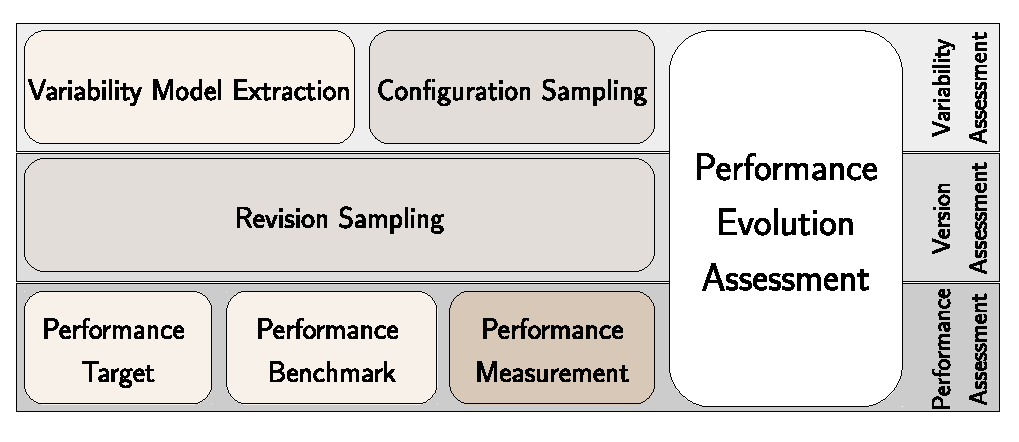
\includegraphics[width=0.75\textwidth]{images/process_overview.eps}
	\caption{Overview of the the proposed methodology including the necessary processes.}
	\label{fig:overview}
\end{figure}

First, objectives related to the variability of a configurable software system
are considered. This includes the extraction and comprehension of knowledge
about the system’s variability. Second, we address objectives which emerge with
evolving software, for instance whether a system compiles for a specific
version, or whether a version is a promising candidate for detecting
performance changes. Finally, we describe in detail the assessment of
performance which comprises the selection of suitable performance benchmarks as
well as a selection of appropriate statistical means to summarize, compare, and
evaluate performance statistics in order to derive meaningful insights.

In addition to the three aforementioned dimensions in Figure~\ref{fig:overview},
performance evolution assessment can also be conceived as consisting of three different
categories of tasks, as the different colorizations indicate. 
First, for a configurable software system, its variability needs to be
assessed in order to obtain a variability model to derive and
select configurations from.
Second, for a software system, a sample set of revisions needs to be selected.
Since covering all variants and versions is not feasible, a sampling strategy needs to be chosen
which is likely to uncover performance changes. Finally, the
performance assessment goals are specified and corresponding
measurements are conducted and evaluated as mentioned above.


\chapter{Background and Related Work}\label{chapter:2}
This chapter is intended to recapitulate the background of the thesis theme. In
Sec.~\ref{sec:2.1}, we recall the evolution of software systems with respect to
architecture and variability. In Sec.~\ref{sec:2.2} we outline the characteristics
of software performance, practical testing and measurement strategies as well as
some statistical background necessary to analyze, interpret and compare
performance assessment. In Sec.~\ref{sec:2.3} we present recent approaches for
feature model extraction from existing software systems and code artifacts. Finally, in
Sec.~\ref{sec:2.4} we recall and compare in detail different approaches to model
and predict performance behavior for configurable software systems.

\section{Variability Modeling}
{\color{violet}
The design and development of configurable software systems is conceptually
divided into \emph{problem space} and \emph{solution space} \citep{czarnecki_generative_2000}. The problem space
comprises the abstract design of features that are contained in the software system as well as
constraints among features, such as dependencies or mutual-exclusion. The
solution space describes the technical realization of features and the
functionality described by and associated with features, e.g., implementation
and build mechanisms. That is, features cross both spaces since they are mapped
to corresponding code artifacts.}

A common way to express features and constraints in the problem space is to
define a \emph{variability model}, or \emph{feature model}, which subsumes all
valid configurations
\citep{kang_feature-oriented_1990,apel_feature-oriented_2013}. There are different and equivalent syntactical approaches to define feature models, for instance, a propositional formula $F$ over the set of
features of the configurable software systems \citep{batory_feature_2005}. In
this case a configuration is valid with respect to the feature model if and only if $F$ holds for all
selected features being true and all unselected features being false respectively. 
However, a more practical and more commonly used way to express feature models
are graphical tree-like \emph{feature diagrams}
\citep{apel_feature-oriented_2013}. In a feature diagram, features are ordered
hierarchically, starting with a root feature and subsequent child features. By
definition, the selection of a child feature requires the parent feature to be
selected as well. Child features can either be labeled as \emph{optional}
features  or \emph{mandatory} features; the latter ones need to be selected in
every valid configuration.
Moreover, feature diagrams
provide a syntax for two different types of feature groups, \emph{or-groups} or
\emph{alternative-groups}. For an or-group at least one of the group's features
needs to be selected for a valid configuration, whereas for an alternative group
exactly one out of the group's mutually exclusive features must be selected. In
addition to the feature hierarchy, constraints, which cannot be expressed by
the tree-like structure, are referred to as \emph{cross-tree constraints}.
Cross-tree constraints, depending on the notation, are depicted by arrows
between two features or simply added to the feature diagram as a propositional
formula. For such two features $f_1$ and $f_2$, a cross-tree constraint means
that for feature $f_1$ to be selected, either the selection of $f_2$ is
required/implied or excluded.

An introductory example for the syntax and semantics of feature diagrams is
provided in Fig.~\ref{fig:introduction_fm}. In this example an imaginary
vehicle propulsion can be configured with eight valid configurations. The vehicle requires an engine,
thus, feature \textsf{Engine} is mandatory. At least one out of the three
features \textsf{Hybrid}, \textsf{Piston} and \textsf{Electric} needs to be
selected. For a piston engine, we can select either the feature \textsf{Diesel}
or \textsf{Petrol}. A petrol engine requires additional ignition sparks in
contrast to a Diesel engine. For an electric engine we require a
battery, hence, the feature \textsf{Battery} is mandatory.
In addition, the feature model specifies two cross-tree constraints: First, the
feature \textsf{Tank} is optional, yet once a piston engine is selected, we
require  a tank. Second, if we want to use the \textsf{Hybrid} functionality
(e.g., use both electric and piston engine simultaneously), we require to have both a piston
and an electric engine.

\begin{figure}[htbp]
  \centering
  
  	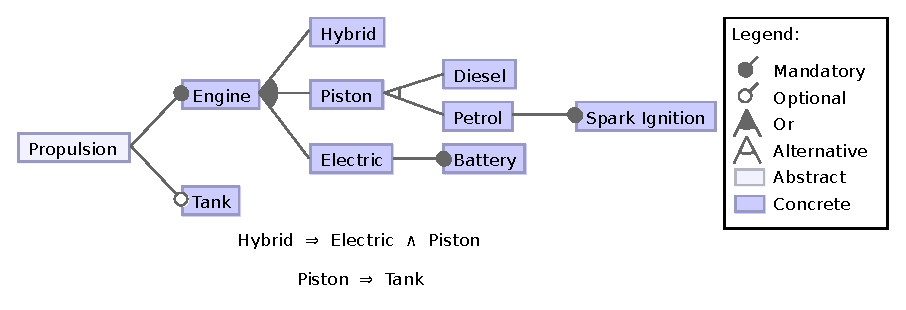
\includegraphics[width=0.85\textwidth]{images/introduction_fm.eps}
  \caption{Feature diagram for a feature model with eight valid configurations;
  two cross-tree constraints are specified as propositional formulas over
  features}
  \label{fig:introduction_fm}
\end{figure}

\section{Evolving Software} \label{sec:2.1}
\subsection{Software Evolution}
The first notion of a software systems' development process is usually
developer-centered and merely focuses on software being designed, implemented,
tested and eventually being released and deployed. Maintainability is a
generally recognized software quality property to look after, and maintenance
is, of course, essential to every successful software system. Nonetheless, less
attention is given to the ability to adapt a software system to changing
requirements (evolvability) rather than maintaining it to keep functionality
working \citep{parnas_software_1994}. Software evolution and evolvability, like
software itself are manifold. Software evolves in many ways ranging from maintenance (refactoring,
bug-fixes and patches) to adapting to changed requirements (adding, removing,
reorganizing functionality and variability).

Modern software systems not only often ship with a variety of configuration
options to select, they also employ routines to be build and sometimes even
make use of or are part of platforms, such as apps or plugins. That is,
software evolution affects all aforementioned aspects and maintainability as
well as evolvability can degrade as software evolves.

\subsection{Software Erosion}
The negative symptoms of software evolution, which are referred to as
``architectural erosion'' \citep{breivold_systematic_2012}, have
been addressed by many researchers.
Most of existing research so far though focuses on evolution regarding software architecture
\citep{breivold_systematic_2012}. The main driving factors leading to symptoms of decay
identified by \cite{perry_software_1991} are architectural erosion and
architectural drift. While architectural drift subsumes developers'
insensitivity when not following a systems architecture or respective guidelines while making changes, architectural erosion subsumes ignoring and violating the existing software
architecture. \cite{parnas_software_1994} argues that as software evolves, software is maintained
and evolved by developers who are not necessarily familiar with the initial
architectural design and, therefore, knowledge about the architecture becomes
unavailable. Although the unfavorable effects of software evolution do not necessary break a
system necessarily and imminently, the software becomes ``brittle'' \citep{perry_software_1991}
as maintainability as well as evolvability degrade. Concrete  symptoms of software
erosion on the implementation level have been documented. 

\cite{zhang_variability_2013} have studied erosion symptoms for a large-scale
industrial software product line with compile-time variability using
preprocessor directives.
They identify variability-related directives and clusters of those to tend to become more
complex as the software evolves. The negative effects, or symptoms of software
erosion are described as, but not limited to \emph{code replication} or
interdependencies between code elements, such as \emph{scattering} and
\emph{tangling}. Code scattering describes the phenomenon of code belonging to
a certain feature being scattered across multiple units of implementation,
e.g., modules, whereas code tangling means that code from different and
potentially unrelated features in entangled within a single module.

\cite{passos_feature_2015} have studied the extent of usage of scattering for device-drivers
in the Linux kernel. Despite scattering being quite prevalent, their
findings suggest that the kernel architecture is robust enough to have evolved
successfully. Nonetheless, platform drivers in the Linux kernel seem more
likely to be scattered than non-platform driver. They conclude that this is a
trade-off between maintainability and performance: a more generalized and
abstract implementation for platform-drivers in this case could possibly avoid
scattering, yet refactorings in this manner did not seem to be necessary or
worth the effort yet.

\subsection{Variability Evolution}
Apart from architecture evolution, the variability offered by software systems
evolves as well. For configurable software systems (or software product lines; 
these terms are not equivalent, but every SPL is a configurable software system)
evolution steps will not only affect artifacts in the solution space, yet also be visible in changes in the respective variability models.
Although the variability aspect of software evolution has not been drawn as
much attention to as has been on architecture in the past, more and more
research has emerged recently to address and understand variability evolution.

\cite{peng_analyzing_2011} proposed a classification of variability evolution patterns that
conceives evolution as adaption to changing (non-)functional requirements as
well as changing contexts. For a context in that sense, two
categories exist. A driving context determines, whether a variability model and respective variants
can meet functional requirements in the first place. A supporting context by
definition determines how non-functional properties are strengthened or
weakened. Any changed requirement is likely to change the contexts for a
software systems variability model and, therefore, will make adaptations of the
variability model necessary. Within their classification method Peng et al.
identify  major causes for variability evolution, comprising a) new driving
contexts emerging, b) weakened supporting contexts (for instance, due to new
non-functional requirements), and c) unfavorable trade-offs for non-functional
properties. 

To understand single evolutionary steps, several catalogs of variability
evolution patterns have been proposed. \cite{peng_analyzing_2011} present three patterns,
where either a new feature is added, a mandatory feature becomes optional, or a
mandatory/optional feature is split into alternative features. \cite{seidl_co-evolution_2012} suggest a catalog of
patterns for co-evolution of variability models and feature mappings that additionally introduces code clones, splitting a feature
into more fine-grained sub-features and feature removal as evolution patterns.
In addition, \cite{passos_towards_2012} have studied variability evolution in
the Linux kernel and present a catalog of patterns where features are removed from the
variability model, but remain a part of the implementation. Their
catalog, among others, includes feature merges, either implicit (optional feature merged
with its parent) or explicit.

The classification proposed by \cite{peng_analyzing_2011} is a general and formalized approach
that, as well as \cite{seidl_co-evolution_2012} and \cite{passos_towards_2012}, describes
elementary evolution patterns which can be composed to more complex patterns. Nonetheless, no
comprehensive catalog of variability evolution so far has been proposed as all
mentioned work above focuses on those patterns that appeared to be relevant for
the respective case study.

\section{Feature Model Synthesis}  \label{sec:2.3}
A variability model as an abstraction of functionality of a software system is
required, or at least of great interest, in many contexts. \emph{First}, not
every configurable system (or software product line) provides an explicit
representation of its variability model. 
The reasons for inexplicit or absent configuration specification are manifold.
They can range from poor or inconsistent documentation
\citep{rabkin_static_2011}, overly complex configurability \citep{xu_hey_2015}
or configuration constraints originated in different layers of a software
system, e.g.m build constraints  or compiler constraints \citep{nadi_where_2015}. 

\emph{Second}, variability models have emerged to be a useful means in domain
and domain analysis prior to developing a software system. As variability
models group and organize functionality, synthesizing a variability model has
shown to be applicable to extract features and constraints from functional
requirements. In addition, by comparison of product specifications for an
existing market domain, variability models can provide detailed feature summary.

For this thesis, we focus on the first aspect of synthesizing variability
models, as our work addresses the assessment of already existing configurable
software systems. Nonetheless, many techniques employed in the aforementioned
second aspect address similar problems, yet rely on natural language artifacts
rather than code artifacts \citep{alves_exploratory_2008,bakar_feature_2015}.
The following section recalls work on extracting configuration options and
constraints from source code as well as the organization of constraints into
feature hierarchy and groups. The further assessment of configurable systems
requires a well-defined and sound variability model.

\subsection{Feature Extraction} 
The first objective in recovering a variability model from a configurable
system is to determine the set of available configuration options to select. In
addition, for further configuration the type of each configuration option
(e.g., boolean, numeric or string) and the respective domain of valid values
needs to be specified.

\cite{rabkin_static_2011} proposed a static, yet heuristic approach to extract
configuration options along with respective types and domains. They exploit the
usage of configuration APIs. Their approach works
in two stages and commences with extracting all code sections where
configuration options are parsed. Subsequently, configuration names can be
recovered as they are either already specified at compile-time or can be
reconstructed using string analysis yielding respective regular expressions.
Moreover, they employ a number of heuristics to infer the type of parsed
configurations as well as respective domains. First, the return type of the
parsing method is likely to indicate the type of the configuration option read.
Second, if a string is read initially, the library method it is passed to can
reveal information about the actual type. For instance, a method
\emph{parseInteger} is likely to parse an integer value. Third, whenever a
parsed configuration option is compared against a constant, expression or value of an enum class,
these might indicate valid values or at least corner cases of the configuration
options' domain. The extraction method by \cite{rabkin_static_2011} renders to be precise, but is
limited, for instance, when an option leaves the scope of the source code.
Nonetheless, for the systems they evaluated they recovered configuration
options that were not documented, only used for debugging or even not used at
all.

\subsection{Constraint Extraction}
The second, or an additional step in recovering a variability model is the
extraction of configuration constraints. An approach proposed by \cite{zhou_extracting_2015}
focuses on the extraction of file presence conditions from build files using symbolic execution. A more comprehensive investigation of configuration
constraints and their origin is provided by \cite{nadi_mining_2014,nadi_where_2015}. They
propose an approach based on variability-aware parsing and infer constraints by
evaluating make files and  analyzing preprocessor directives. Inferred
constraints result from violations of two assumed rules, where a) every valid
configuration must not contain build-time errors and b) every valid
configuration should result in a lexically different program, thus. While the
first rule aims at inferring constraints that prevent build-time errors, the
second one is intended to detect features without any effect, at least as part
of some configurations. Their analysis one the one hand emerged to be accurate
in recovering constraints with 93~\% for constraints inferred by the first rule
and 77~\% for second one respectively. On the other hand, their approach was
only to recover 28~\% of all constraints present in the software system.
Further qualitative investigation, including developer interviews, lead to
the conclusion that most of existing constraints stem from domain knowledge.

\subsection{Feature Hierarchy Recovery} 
Besides recovering configuration options and respective constraints, to reverse
engineer a feature model, one further step is required. The recovered knowledge
needs a tree-like hierarchy, detection of feature groups and cross-tree
constraints to be an acceptable feature diagram
\citep{kang_feature-oriented_1990}. While several approaches to the recover feature model hierarchy have been proposed,
we are primarily interested in finding a hierarchy for knowledge obtained from
source code. Other scenarios, as already stated in the opener of this section,
are based on product descriptions or sets of valid configurations. The remainder of
this subsection we will focus on organizing features and constraints extracted
from source code. For further reading \cite{andersen_efficient_2012} present algorithms
for structuring feature diagrams for three different scenarios including the
ones previously mentioned.

Given an extracted set of features along with corresponding descriptions and
recovered constraints among the features, \cite{she_reverse_2011} propose an
semi-automated and interactive approach to synthesize a feature hierarchy.
Their approach comprises three steps: 1) Specifying a feature hierarchy, 2)
detecting and selecting feature groups, and 3) adding a cross-tree constraint
formula to the feature  model.

\begin{enumerate}
  \item Their approach commences with finding a single parent for each
  feature and, thus, specifying a tree-like feature hierarchy. Based on the
  given constraints a directed acyclic graph (DAG) representing implication
  relationships among features, a so-called implication graph, is constructed:
  Every vertex depicts a feature and edges are inserted for each pair of
  features $(u, v)$, where  $u \implies v$ holds with respect to the given
  constraints.
   
  In addition to the implication graph, the algorithm for each feature computes
  two rankings of features that are likely to be the respective parent feature.
  The two rankings both employ the feature descriptions. Feature descriptions
  are compared for similarity using a similarity metric. For two features $p$
  and $s$ the similarity is defined as the weighted sum of the inverse document
  frequencies $idf(w)$ for the words that the descriptions of features $u$ and
  $v$ share.
  The idf-ranking for a word $w$ is the logarithm of the number of features
  divided by the number of features whose description contains $w$. Each $idf$
  value is weighted by with by the frequency of $w$ in the description of
  feature $p$.
  
  The first ranking, called Ranked-Implied-Features (RIF), for each feature $f$
  ranks features by their similarity to $f$ in an descending order, but
  prioritizes those features that are implied according to the previously
  computed implication graph. The second ranking, called Ranked-All-Features
  (RAF) is similar to RIF, yet less strict since implied features are not
  prioritized. Given these ranking, a user selects for each feature a suitable
  parent feature from the RIF or RAF ranking. The idea behind providing two
  separate rankings, according to \cite{she_reverse_2011} is that the given
  extracted constraints can be incomplete and, thus, not all relevant implications are
  contained.

  \item After the feature hierarchy is specified, another auxiliary graph, a
  mutex graph, similar to the implication graph, is constructed. The mutex
  graph is an undirected graph with features as vertices and edges between two
  features $u$ and $v$, if $u \implies \neg{v}$ and $v \implies \neg{u}$ hold
  with respect to the given constraints. That is, all incident adjacent are mutually exclusive. Based on
  this mutex graph all maximal cliques (subsets of vertices that all are
  connected with each other) among the vertices with the same parent are
  computed. Those cliques are mutually exclusive and share the same parent and
  represent mutex- or alternative-groups. \cite{she_reverse_2011} introduce an
  additional constraint to extract xor-groups that require one of the groups’
  features to be selected if the parent is selected. This distinction is in
  line with the initial description of feature diagrams by \cite{kang_feature-oriented_1990},
  but not all descriptions follow this distinction between mutex- and
  xor-groups and just use the term alternative-group mentioned in Sec. 1.
  
  \item The cross-tree constraints for the feature diagram are extracted from
  the given configuration constraints. Since CTCs are constraints that could
  not be represented by the feature hierarchy (implication) or
  alternative-groups (exclusion) the derivation of CTCs follows this idea. The
  set of cross-tree implications is derived by removing all edges that are part
  of the feature hierarchy from the initially constructed implication graph.
  The set of cross-tree exclusions is derived in the same manner from the mutex
  graph by removing all edges among vertices of all mutex-groups. To make the
  feature model sound, the given configuration constraints, reduced to those
  clauses that are not already entailed by the diagram, can be added as an
  additional CTC formula to the feature diagram.
\end{enumerate}

The approach by \cite{she_reverse_2011} provides a practical algorithm to synthesize a
feature diagram, yet has some aspects we might need to consider. First, the
approach is not able to detect or-groups as defined in Sec. 1. Second, the
approach does introduce a root feature. Finally, the approach does not
distinguish between mandatory and optional features. Implicitly, all features
that do not have a parent feature are optional and all features that have a
parent feature are by default mandatory. \cite{she_reverse_2011} evaluated the
algorithm with both complete and incomplete variability knowledge (feature
names, descriptions and constraints). While the algorithm emerged to be
practical, detecting features whose parent was the root-feature was difficult.

\section{Assessing Performance} \label{sec:2.2}
While the last three sections covered software evolution and variability
modeling, we know step forward to the topic of software performance. This
section will the outline performance with respect to software systems as well
as to possible measurements. We provide a brief look at the general performance
testing setup and the required prerequisites, including suitable benchmarks.
Finally, we provide the statistical background to summarize, interpret and
compare performance measurements accurately.

\subsection{What is Performance?}
The performance of software systems is, like software quality, primarily a
matter of perspective. While an end user might consider practical aspects to be
more important, from a developer’s perspective, performance relates to and is
best described by non-functional properties \citep{molyneaux_art_2014}. While
functional properties subsume what exactly a software system does, non-functional
properties describe how (good or bad) a software system is at providing the
functionality offered. The notion of good and bad in this sense corresponds to
non-functional requirements (NFR), that is, software with good performance
behavior satisfies NFRs. The categories of NFRs what shape performance behavior
are manifold. According to \cite{molyneaux_art_2014}, \emph{key performance
indicators} (KPIs) include 

\begin{itemize}
  \item availability
  \item response time,
  \item resource utilization, and in a broader scope also 
  \item capacity.
\end{itemize}

Time-related KPIs are availability and response time, whereby
availability describes the time or time ratio that the software is available to
the end user and response time subsumes the time it takes to finish a request
or operation. Throughput as a category subsumes the program behavior with
respect to program load, such as hits per second for a web application or
amount of data processed per second. Resource utilization describes the extent
to which a software system uses the physical resources (CPU time, memory, and
disk or cache space) of the host machine. Finally, from a web-centered
perspective, capacity describes measurements with respect to servers and
networks, such as network utilization  (traffic, transmission rate) and server
utilization, such as resource limitations per application on a host server.

Consequently, the assessment of performance requires a context or testing
target that corresponds to the assesses system under test (SUT). For instance,
for a simple command-line compression tool, suitable KPIs are response time and
throughput, whereas performance for an online shop web application is better
outlined by availability and capacity.

\subsection{Performance and Software Engineering}
In the last section we referred to performance, or in detail, the KPIs, as
possible testing targets we validate against non-functional requirements.
However, in a broader sense software performance has become a facet of software
engineering and a lot of effort has been spent to study, describe, and improve
performance. Performance assessment in a software engineering context,
according to \cite{molyneaux_art_2014}, comprises a number of activities that
are related to or part of software development: Besides the analysis of concerns or
requirements with respect to performance, software performance engineering
entails performance testing and prediction and can contribute to maintenance
and evolution aspects \citep{woodside_future_2007}. While performance testing,
like other testing targets, is intended to validate requirements, prediction aims to
approximate performance behavior measures for different scenarios or
configurations. Moreover, performance behavior predictions can help anticipate
the impact of various changes \citep{woodside_future_2007}.
The authors, moreover, present the two approaches in assessing software
performance. So-called model-based approaches aim to describe performance
behavior by modeling functionality, for instance, modeling scenarios in UML,
using performance estimations early in the development process. In contrast to
that, accommodated later in the development process, measurement-based
approaches aim to model performance behavior based on measurements of existing
prototypes. The latter class of performance assessment includes classical
performance (regression) testing. The authors, moreover, outline the
anticipated future of both approaches and advocate the combination or
convergence of both approaches in the future. Since then, especially more
measurement-based performance prediction approaches have emerged. More on this
in the next section, the remainder of this subsection will outline the general
performance testing setup.

\subsection{Performance Testing}
The first step in performance testing, prior to defining relevant KPIs and
metrics, is to specify a system operation or use case \citep{woodside_future_2007} to
validate. A typical use case includes a well defined task or workload to
process, expected behavior or and outcome or state, and performance
requirements as previously discussed. For the SUT, however, we require a
version that does compile or, in case it is interpreted, is syntactically
correct \citep{molyneaux_art_2014}. With regard to performance assessments as part of
the development process, a code freeze should be obtained since measurement
results are likely to become meaningless for later versions. In addition to
that,  the machine or setup used for performance measurement should ideally be
as close to the production environment as possible, but at least be documented
to compare different runs.

Finally, one or more benchmarks need to be selected to simulate  the program
load for the respective use case. A benchmark, all in all, needs to be
representative, i.e., should relate to the the use case or requirement one
 wants to validate. While benchmarks for file compression usually include
multiple different types of media data (text, sound, pictures) like the
Canterbury corpus, web applications can be exposed to dealing with a number of
simulated users at the same time \citep{molyneaux_art_2014}. Benchmarks have often been
standardized within research and engineering to provide comparable performance
measurements. A popular examples is the Software Performance Evaluation
Corporation (SPEC), a consortium providing a variety of benchmarks like the
CPU2000 processor benchmark consisting of both floating point and integer
operations. Nonetheless, benchmarks in a sense of repeatable program load can
be obtained from load generation software like ApacheBench for the Apache web
server or simply by measuring performance for test cases.

Performance testing heavily relies on tool support, especially for repeating
test cases, recording measurements, and dynamic program analysis. While the
tool solutions for performance testing vary from domain, scale and purpose, we
will only outline the general tool architecture. \cite{molyneaux_art_2014} describes
four primary components: a scripting module, a test management module, a load
injector, and an analysis module. A scripting module handles the generation or
repetition of use cases which, for instance, can be recorded prior to the test
for web applications. A test management module creates and executes a test
session, whose program load is generated by one or more load injectors. A load
injector can provide a benchmark or generate items to process or can simulate a
number of clients for a server-side application. An analysis module, finally,
collects and summarizes data related to the performance testing target. More on
summarizing and comparing recorded results in the next section.

\subsection{Statistical Considerations}

\begin{itemize}
  \item Arithmetic mean: $$\text{a-mean} = \frac{1}{n}\sum_{i=1}^{n} X_i$$
  \item Geometric mean: $$\text{g-mean} = \bigg(\prod_{i=1}^{n}
  X_i\bigg)^\frac{1}{n} = \sqrt[\leftroot{-2}\uproot{2}n]{X_1 X_2 \ldots X_n}$$
  \item Harmonic mean: $$\text{h-mean} = n \cdot \bigg(\sum_{i=1}^{n}
  \frac{1}{X_i}\bigg)^{-1}$$
\end{itemize}

\section{Performance Modeling} \label{sec:2.4}
\begin{itemize}
  \item Genetic algorithms \citep{guo_genetic_2011}
  \item Variability-aware modeling \citep{guo_variability-aware_2013}
  \item via feature-interaction and performance influence models
  \citep{siegmund_predicting_2012,siegmund_performance-influence_2015}
\end{itemize}

\chapter{Methodology: Variability Assessment}\label{sec:chapter:3}
To assess performance evolution for configurable software systems, it is
required to assess and understand variability of such systems with respect to
various aspects: \emph{First}, to actually assess single variants, knowledge
about the variability model is required to configure the software systems accordingly.
\emph{Second}, obtaining knowledge about feature usage and implementation can
provide meaningful insights. For instance, knowing that most variable code is dependent
on small numbers of features might be useful information when selecting a
sampling strategy. Similarly, knowing which feature combinations are frequently
involved in conditioning program functionality and behavior can help understand
configuration-related defects. \emph{Last}, since the number of configurations
for most configurable software systems is infeasible, variability assessment faces
performance- and scalability-related problems. That is, variability assessment
is usually constrained by limited resources.

\begin{figure}[h!]
	\centering
	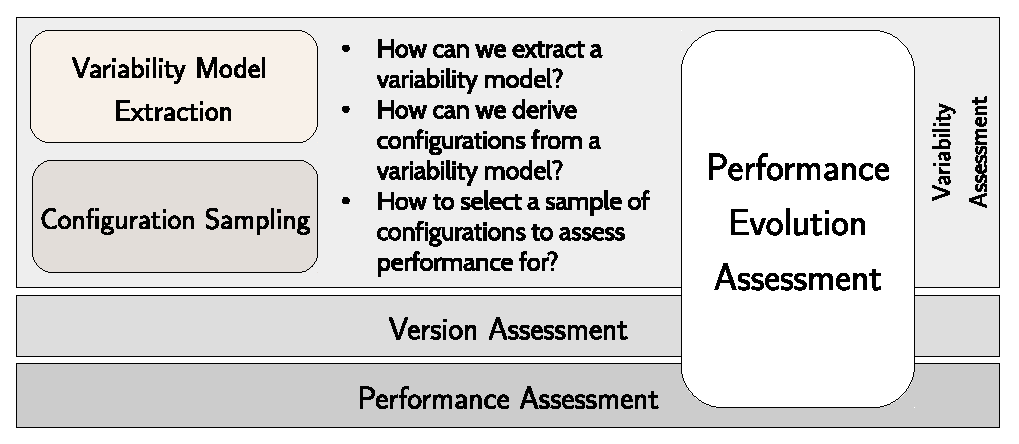
\includegraphics[width=0.99\textwidth]{images/process_varassesment.eps}
	\caption{Methodological roadmap: questions to address during variability
	assessment.}
	\label{fig:roadmap_1}
\end{figure}
 
This chapter describes the first aspect in our methodology, the assessment of
variability. As illustrated in Figure \ref{fig:roadmap_1}, this first tier of
our methodology embraces two main tasks, first, the synthesis (or extraction) of a variability model for a configurable software system, and second, strategies to select
meaningful sample sets of configurations to assess performance for. In
section~\ref{sec:untangling} we review the synthesis of variability models as
well as corresponding analyses of systems’ variability; in
section~\ref{sec:configuration_gen} we describe means to generate configurations from variability models, and finally,
section~\ref{sec:configuration_sam} discusses different strategies for selecting
sample sets of configurations.

\section{Untangling Variability}\label{sec:untangling}
Before presenting strategies to synthesize variability models in
the next section, we first recap a number of techniques to untangle configurable
software composed from variable and invariant code. In the context of our
methodology, these techniques are useful means to make variable code segments
visible, and to understand how variability influences the overall resulting
variants of a software systems.
The idea of designing and developing configurable software systems is driven by
the separation of different concerns, expressed as features of a software
system. A configurable software system is either assembled at compile-time with
respect to its configuration, or tailored to a configuration at
load-time \citep{apel_feature-oriented_2013}. Both ways of implementing the
variability exist in practice.
Research has also proposed a variety of variant-generating implementation techniques for
compile-time variability, ranging from simple preprocessor directives to
features as separate modules \citep{kastner_model_2009}.  A complete survey of means to implement
configurable software systems would likely exceed the scope of this section, yet we intend to discuss in this
section which information regarding variability is required or useful to our
methodology, and how it can be obtained.

\subsection{Family-based Analyses}
As the number of variants for configurable software systems is usually
infeasible, naive analyses of configurable systems are not trivial. Any static
analysis can only assess one variant at a time, as well as dynamic analyses,
which can follow only one execution path. 
In contrast to that, recently,
extended analysis techniques, which are aware of variability of the systems
studied, have emerged \citep{thum_classification_2014}. In particular, these
\emph{family-based} analyses avoid redundant computation, such as visiting a
code section multiple times, and exploit artifacts shared by multiple variants
\citep{thum_classification_2014}. Besides more efficient analysis, family-based
methods incorporate knowledge about valid feature combinations
\citep{thum_classification_2014} and, therefore, connect analysis results with
a context, such as feature combinations, for which the findings hold.
Family-based methods have been widely used across various domains and can
provide useful information when assessing configurable software systems.

\paragraph{Variability-aware Parsing.} \cite{kastner_variability-aware_2011}
have proposed the framework \emph{TypeChef} to enable the construction of
variability-aware parsers. A variability-aware parser, like ordinary parsers,
systematically explores a program to return an abstract representation of the
parsed program. This parse tree, or abstract syntax tree,
is the basis for compilers to translate a program, or for further static
analyses, such as type checking. For a code base with variability expressed by
preprocessor annotations, which are evaluated prior to compilation, a
variability-aware parser, however, is able to derive a parse tree considering
all variants in a single run. A parse tree usually consists of nodes
representing syntactical features of the parsed program. The parse tree
returned by a variability-aware parser, moreover, comprehends variable segments
of a program and will include them with respect to their presence conditions.
For instance, a class may contain a function \textit{sort()}, for which two
different implementations exist. While there might be numerous variants, the parse tree
of the class will contain a node with two children, one for each
implementation; higher numbers of alternative implementations are expressed by
nesting further nodes. In that way, variable and invariant program segments
can be separated.

While the approach of \cite{kastner_variability-aware_2011} handles
undisciplined usage of preprocessor directives, such as splitting function parameter lists, variable types, or
expressions, \cite{medeiros_discipline_2017} have proposed an approach to avoid and
conservatively refactor those cases. The authors propose a catalog of
refactoring templates, which describe transformations from undisciplined usage
of preprocessor annotations to disciplined ones. With respect to
variability-aware parsing, disciplined usage is conceived as using preprocessor
annotations only to segment statements, but not to segment a single syntactical
unit, such as expressions \citep{medeiros_discipline_2017}.

In the context of our methodology, the parse tree resulting from
variability-aware parsing can be used as a basis for further analyses. Since
the parse tree provides a machine-readable decomposition of variable and
invariant code segments along with presence conditions, for instance, it has
been used to derive constraints among features
\citep{nadi_mining_2014,nadi_where_2015} as we will see in the next subsection.

\paragraph{Staged Variability.} Besides variability-aware parsing,
\cite{nguyen_building_2014} have applied symbolic execution
\citep{king_symbolic_1976,darringer_applications_1978} to unwind variability for
PHP Web applications. Web applications are staged, i.e., even though they can be
configured at load-time, the application is as well variable with respect to
input received at run-time. For instance, consider \emph{WordPress}, a popular
content management system (CMS) implemented in PHP, which can be extended with a number
of plug-ins. However, the content of a website presented to the user also depends
on information retrieved from a database, and user input. Consequently, a
dynamic PHP Web application is staged in a sense that it generates configurable
HTML templates which are rendered at run-time. The authors utilize a symbolic
execution engine to explore all possible execution paths. Each user input or
database query is considered a symbolic value which is propagated through each script.
By keeping track of the (partially symbolic) HTML output and organizing it in a
DOM-like structure, their approach approximates the HTML output, which
subsequently can be tested, for instance for validity
\citep{nguyen_auto-locating_2011}.
Similarly, \cite{lillack_tracking_2014} have applied taint-analysis to configurable software
systems to track the influence of configuration options read at load-time.
Their static analysis approach taints every value resulting from reading a
configuration parameter as well as every value resulting from a computation
that involves previously tainted values. That way, lines of code that are
possibly depending on configuration options are detected.

In the context of our methodology, addressing staged variability with techniques
such as symbolic execution is required to assess performance for Web
applications. Both the code executed at server-side as well as the dynamically
generated HTML are interdependent parts of the Web application. Any suitable and
elaborate performance measurement setup for Web applications must incorporate
both stages.

\paragraph{Build System Variability.} Apart from
configuring software systems using preprocessor annotations, the assembling of
a configurable software system can as well be orchestrated by its underlying
build system. While preprocessor annotations virtually separate code fragments
of different features, for instance, build systems can physically exclude files
from compilation. This implementation of variability enabled by build systems,
in particular of Makefiles, has been subject to a couple of analysis approaches.
\cite{tamrawi_build_2012} have proposed \emph{Symake}, a symbolic execution
engine to evaluate Makefiles.
On top of \emph{Symake}, \cite{zhou_extracting_2015} utilize symbolic execution
to analyze Makefiles and derive file presence conditions, stating under which feature
selection a file is included or excluded from compilation. The work of
\cite{al-kofahi_escaping_2016} addresses a more advanced build system, \emph{GNU
Automake}. \emph{Automake} describes a staged build process, where a Makefile
can be specified on a higher level, and is subsequently compiled to an actual Makefile. The
authors’ aim to provide a variability-aware representation of all possible
Makefiles to enable further analyses of the build process.

In the context of out methodology, the symbolic evaluation of a software
system’s build process follows an intention similar to the one of
variability-aware parsing. Not only could further analysis tools be build upon
a symbolic evaluation engine, but also does symbolic evaluation in this context
untangle the variability accommodated in the build process. The file presence
conditions extracted by \cite{zhou_extracting_2015}
and \cite{al-kofahi_escaping_2016} are a strong basis for further constraint
extraction, and therefore variability model assessment.\\

In the context of our methodology, the mentioned family-based analyses serve two
fundamental purposes. \emph{First}, family-based analyses can help to obtain an
overview of what, or how much code in a configurable software system is variable
as well as to which extent.
For instance, if most extracted presence conditions contain only very few
features, higher-order feature interactions are unlikely. \emph{Second},
family-based analyses provide a feasible means to untangle variability and, as we will see in the
next section, are the basis for some elaborate techniques to extract
variability models \citep{nadi_mining_2014,nadi_where_2015}. In conclusion,
these analyses are not essential to extract variability models, yet are useful tools to use in
addition to the strategies mentioned in the next section.

\subsection{Variability Model Synthesis} \label{sec:feature_model_synthesis} 
A variability model as an abstraction of functionality of a software system is
required, or at least of great interest, in many contexts. Not every
configurable system provides an explicit representation of its variability
model. The reasons for inexplicit or absent configuration specification are
manifold. They can range from poor or inconsistent documentation
\citep{rabkin_static_2011} to overly complex configurability
\citep{xu_hey_2015}, or configuration constraints originated in different layers of a software system,
such as build constraints or compiler constraints
\citep{nadi_mining_2014,nadi_where_2015}.
The following paragraphs review different \emph{strategies to synthesize
variability models} from different types of artifacts. A classification of
strategies, along with corresponding literature is illustrated in
Figure~\ref{fig:varsynth_overview}.

The first category comprises extraction based on Natural Language Processing (NLP) utilize
similarities between textual representations of different variants to derive
common features \citep{alves_exploratory_2008,bakar_feature_2015}. The
approaches in the second category are heuristics based on static analyses, whereby configuration option names \citep{rabkin_static_2011} are
extracted, or constraints are derived from assessing the software’s build
process \citep{nadi_mining_2014,nadi_where_2015}. The last category comprises
techniques which conceive variability model as an optimization problem. For a set of given and
valid configurations, genetic algorithms are used to approximate an optimal
feature model representing constraints among features 
\citep{lopez-herrejon_reverse_2012,lopez-herrejon_assessment_2015,linsbauer_feature_2014}.

\paragraph{NLP-based Extraction.} As feature diagrams group and organize
features (representing functionality), synthesizing a variability model has shown to be applicable to extract features
and constraints from natural language artifacts. For instance, by comparing
product specifications for an existing market domain, variability models can
provide a detailed feature summary \citep{alves_exploratory_2008}.

The basic idea is to identify commonalities and differences in natural language
documents, such as product descriptions, requirements, or documentations, by
using natural language processing (NLP) techniques \citep{bakar_feature_2015}. A
widely employed technique is to conceive a text as a vector in a vector space model, where each word or
token represents a dimension. From the tokenized text, irrelevant stop words
are removed, and all remaining words are reduced to their original word stems.
The importance of all remaining tokens is (usually) weighed by its tf-idf
value, an established technique in information retrieval. That is, each text
(corresponding to a variant or configuration) is represented as a vector of
tf-idf values in the aforementioned vector space model. 
Based on these representations, text instances are clustered to identify
commonalities and differences, for instance in terms of shared words.
Subsequently, the clustering information can be used to extract features or entire feature
models \citep{alves_exploratory_2008,bakar_feature_2015}.

\begin{figure}[h!]
\centering
\begin{tikzpicture}[sibling distance=13em,
  every node/.style = {rounded corners,
    draw, align=center,
    top color=white, bottom color=blue!20},thick,scale=0.95, every
    node/.style={scale=0.95}]
  \node {\sffamily\bfseries Variability Model Synthesis}
    child { node [align=left] {{\begin{tabular}{c}{\sffamily NLP-based
    Extraction} \\
    \citep{alves_exploratory_2008} \\ \citep{bakar_feature_2015}
    \end{tabular}}}} 
    child { node [align=left] {\begin{tabular}{c} {\sffamily Static
    Analyses}\end{tabular}} child { node [align=left] {\begin{tabular}{c}
    {\sffamily Feature Extraction} \\
    	\citep{rabkin_static_2011}
    	\end{tabular}}} 
    	child { node [align=left] {\begin{tabular}{c} {\sffamily Constraint
    	Extraction}
    	\\
    	\citep{nadi_mining_2014,nadi_where_2015}
    	\end{tabular}}} }
    child { node [align=left] {\begin{tabular}{c} {\sffamily Feature-Model
    Approximation} \\
    \citep{lopez-herrejon_reverse_2012,lopez-herrejon_assessment_2015} \\
    \citep{linsbauer_feature_2014}\end{tabular}}};
\end{tikzpicture}
\caption{Overview of our literature survey on
variability model synthesis.}\label{fig:varsynth_overview}
\end{figure}

\paragraph{Feature Extraction.} \cite{rabkin_static_2011} proposed a static, yet
heuristic approach to extract configuration options along with respective types and domains. Their approach
exploits the usage of configuration APIs and works
in two stages. It commences with extracting all code sections where
configuration options are parsed. Next, configuration names can be
recovered as they are either already specified at compile-time or can be
reconstructed using string analysis yielding respective regular expressions.
Moreover, the authors employ a number of heuristics to infer the type of parsed
options as well as respective domains. \emph{First}, the return type of the
parsing method is likely to indicate the type of the configuration option read.
\emph{Second}, if a string value is read initially, the library method it is
passed to can reveal valuable information about the actual type. For instance, a method
\texttt{parseInteger} is likely to parse an integer value. \emph{Third},
whenever a parsed configuration option is compared against a constant, expression, or value
of an enum class, these might indicate valid values or at least corner cases of
the configuration option domain. The extraction method by
\cite{rabkin_static_2011} is precise, but limited, for instance, when an
option leaves the scope of the source code and is passed to a database.
Nonetheless, for the systems studied, the authors were able to recover
configuration options that were not documented, only used for debugging or even not used at
all.

\paragraph{Constraint Extraction.} 
A more comprehensive investigation of configuration
constraints and their origin is provided by
\cite{nadi_mining_2014,nadi_where_2015}. They use variability-aware parsing to
infer constraints by evaluating Makefiles and  analyzing preprocessor
directives. Inferred constraints result from violations of two assumed rules,
where (a) every valid configuration must not contain build-time errors and (b)
every valid configuration should result in a lexically different program.
While the
first rule aims at inferring constraints that prevent build-time errors, the
second one is intended to detect features without any effect, at least as part
of some configurations. Their analysis has shown a high accuracy
in recovering constraints with 93\,\% for constraints inferred by the first rule
and 77\,\% for second one respectively. However, their approach
recovered only 28\,\% of all constraints present in the software system.
Further qualitative investigation, including developer interviews, lead to
the conclusion that most of existing constraints stem from domain knowledge
\citep{nadi_where_2015}.

\paragraph{Feature-Model Approximation.}
A different strategy to recover variability models, instead of analyzing the
software artifacts, is to approximate a model. Given a selection of valid
feature selections, a variability model best describing the configurations can
be approximated, or learned. \cite{lopez-herrejon_assessment_2015} have surveyed
different search-based strategies to synthesize feature models of which we
present two categories. Evolutionary algorithms have been applied to reverse
engineer feature models from configuration samples
\citep{lopez-herrejon_reverse_2012,linsbauer_feature_2014}. A population of
feature models is generated and each instance is evaluated by a fitness
function, measuring how well it fits the given sample set of configurations.
Subsequently, a new generation is obtained by applying crossover and mutation
operators to the previous generation, whereby only the fittest instances remain.
This process of evolution is repeated multiple times until a desired threshold fitness is reached for a feature model instance.
\cite{lopez-herrejon_reverse_2012} identify a trade-off between the accuracy of
recovered feature models and the number of generations employed by evolutionary
algorithms. Besides promising results, the authors stress the importance of
effective and scalable fitness functions as well as meaningful samples to learn
the feature model from.
Contrary to evolutionary algorithms,
\cite{haslinger_reverse_2011,haslinger_extracting_2013} have proposed an ad-hoc
algorithm to reverse engineer feature models. The algorithm recovers
the feature model layer by layer via extracting all child
features for a given parent feature recursively. The algorithm does not consider
cross-tree constraints.
Besides promising results for basic feature models, the authors advocate the
incorporation of human domain-knowledge in the synthesis of feature models.
 
\paragraph{Feature-Hierarchy Recovery.} \label{sec:feature_hierarchy}
Besides recovering features and their respective constraints, to reverse
engineer a feature model, one further step is required when the outcome should
be human readable in a feature diagram. The recovered knowledge can be
organized in a tree-like hierarchy with feature groups specified and cross-tree
constraints explicitly stated to derive a valid feature diagram
\citep{kang_feature-oriented_1990}.
While several approaches for recovering the feature-model hierarchy have been
proposed, we are primarily interested in finding a hierarchy for knowledge
obtained from source code. In the remainder of this
subsection, we will focus on organizing features and constraints extracted from
source code.

Given an extracted set of features along with corresponding descriptions and
recovered constraints among the features, \cite{she_reverse_2011} propose a
semi-automated and interactive approach to synthesize a feature hierarchy.
Their approach comprises three steps. \emph{First}, an overall feature hierarchy
based on feature implications is specified. \emph{Second}, potential feature
groups are detected and manually selected. \emph{Finally}, the feature diagram
is extended with remaining CTCs. 
The approach by \cite{she_reverse_2011} provides a practical algorithm to synthesize a
feature diagram, yet has some limitations we need to consider. \emph{First}, the
approach is not able to detect or-groups as defined in Sec. \ref{sec:variability_modeling}.
\emph{Second}, the approach does introduce a root feature. \emph{Finally}, the
approach does not distinguish between mandatory and optional features. Implicitly, all features
that do not have a parent feature are optional and all features that have a
parent feature are by default mandatory. \cite{she_reverse_2011} evaluated the
algorithm with both complete and incomplete variability knowledge (feature
names, descriptions and constraints). While the algorithm has shown to be
practical, detecting features whose parent was the root-feature was difficult
since, due to the transitive property of implication, it is implied by each
feature of the feature model.\\

%\begin{enumerate}
%  \item The algorithm commences with finding a single parent for each
%  feature and, thus, specifying a tree-like feature hierarchy. Based on the
%  given constraints, a directed acyclic graph (DAG) representing implication
%  relationships among features, a so-called \emph{implication graph}, is
%  constructed.
%  Every vertex in the implication graph represents a feature  and edges are
%  inserted for each pair of features $(u, v)$, where  $u \implies v$ holds with
%  % respect to the given constraints.
%   
%  In addition to the implication graph, the algorithm for each feature computes
%  two rankings of features that are likely to be the respective parent feature.
%  The two rankings both employ the feature descriptions. Feature descriptions
%  are compared for similarity using a similarity metric. For two features $p$
%  and $s$, the similarity is defined as the weighted sum of the inverse
%  % document frequencies $idf(w)$ for the words that both descriptions of
% features $p$%  and $s$ share.

%  The $idf$-ranking for a word $w$ is the logarithm of the number of features
%  divided by the number of features whose description contains $w$. Each $idf$
%  value is weighted with the frequency of $w$ in the description of
%  feature $p$.
  
%  The first ranking, called Ranked-Implied-Features (RIF), for each feature $f$
%  ranks all features by their similarity to $f$ in an descending order, but
%  prioritizes those features that are implied according to the previously
%  computed implication graph. The second ranking, called Ranked-All-Features
%  (RAF) is similar to RIF, yet less strict since implied features are not
%  prioritized. Given these rankings, a user for each feature selects a suitable
%  parent feature from the RIF or RAF ranking. The idea behind providing two
%  separate rankings, according to \cite{she_reverse_2011} is that the given
%  extracted constraints can be incomplete and, thus, not all relevant
%  implications are contained in the implication graph.

%  \item After the feature hierarchy is specified, another auxiliary graph, a
%  mutex graph, similar to the implication graph, is constructed. The
%  % \emph{mutex graph} is an undirected graph with features as vertices and
%  % edges between two
%  features $u$ and $v$, if $u \implies \neg{v}$ and $v \implies \neg{u}$ hold
%  with respect to the given constraints. 
%  That is, all adjacent features are mutually exclusive. Based on
%  this mutex graph, all maximal cliques (subsets of vertices that all are
%  connected with each other) among the vertices with the same parent are
%  computed. All features within such a clique are mutually exclusive and share
%  the same parent and represent mutex- or alternative-groups.
  % \cite{she_reverse_2011} introduce an additional constraint to extract xor-groups that require one of the groups’
%  features to be selected if the parent is selected. This distinction is in
%  line with the initial description of feature diagrams by
  % \cite{kang_feature-oriented_1990}, but not all descriptions of feature diagrams follow this distinction between
%  mutex- and xor-groups and just use the term alternative-group discussed in 
%  Sec. \ref{sec:variability_modeling}. %2.1
  
 % \item CTCs for the feature diagram are extracted from
 % the given configuration constraints. Since CTCs are constraints that could
 % not be represented by the feature hierarchy (implication) or
 % alternative-groups (exclusion), the derivation of CTCs follows this idea. The
%  set of cross-tree implications is derived by removing all edges that are part
%  of the feature hierarchy from the initially constructed implication graph.
%  The set of cross-tree exclusions is derived similarly from the mutex
%  graph by removing all edges among vertices of all mutex-groups. To make the
%  feature model sound, the given configuration constraints, reduced to those
%  clauses that are not already entailed by the diagram, can be added as an
%  additional CTC formula to the feature diagram \citep{she_reverse_2011}.
%\end{enumerate}

Although the approaches mentioned in the paragraphs above, excluding the
feature-hierarchy recovery, in principal address the same problem, they are
isolated solutions to the problem of variability assessment, and their
applicability is depending on a number of cross-cutting boundary conditions.
\emph{First}, for the overall problem of variability model synthesis we can
identify two different contexts for which different techniques apply. The NLP-based
techniques summarized by \cite{alves_exploratory_2008} and \cite{bakar_feature_2015} address
the extraction of features in the context of requirements engineering, for instance by comparing different
software products in the same market domain. However, the remaining techniques
intend to extract features for a given single software system.
\emph{Second}, for variability assessment there exist two different principal
analysis approaches. While the techniques proposed by \cite{nadi_mining_2014,nadi_where_2015}
and \cite{rabkin_static_2011} approach a configurable software system as a monolithic system,
both the family of NLP-based techniques and the approximative techniques
\cite{lopez-herrejon_reverse_2012,lopez-herrejon_assessment_2015,linsbauer_feature_2014}
explicitly require a set of variants or configurations, respectively.
\emph{Third}, the techniques differ in the type of variability they are able to
extract variability models for. While the approach of
\cite{nadi_mining_2014,nadi_where_2015} only works for build-time variability, the work of
\cite{rabkin_static_2011} will only work for configurations read at load-time. Moreover, the remaining techniques do not consider the different types of
variability at all.

In conclusion, it becomes clear that there is no single textbook solution to
the problem of variability model assessment as this problem may arise in
different contexts be approached from different perspectives, or be emergent
for different types of variability.

\subsection{Methodological Strategies}
The last two subsections reviewed a number of family-based analyses for
configurable software systems as well as approaches proposed to partially
extract variability models from a system’s code base. The latter approaches
presented, however, are rather isolated solutions due to non-generic
assumptions, such as the use of configuration APIs \citep{rabkin_static_2011},
or build-time variability \citep{nadi_where_2015}. At best, these approaches
complement each other, or are an appropriate choice under certain
circumstances, still requiring further manual assessment. The following
integrates the previously discussed work and proposes methodological strategies
to synthesize variability models for different scenarios, or use cases.

For the recovery of variability models, we propose three scenarios. Clearly,
this is not an exhaustive list, but covers the majority of use cases based on
our literature review. The scenarios should provide a practical context to the
previously mentioned techniques. The three scenarios are outlined in Table
\ref{tab:synthesis}; we derive our scenarios based on three criteria.
\emph{First}, we ask whether, and if so, to what extent configurability for a
software system is documented. \emph{Second}, we ask whether the software
system provides sample configurations, such as configuration presets, or
whether it ships as different variants, such as different Windows flavors.
\emph{Last}, we ask whether a variability model is explicitly contained in the
software, and whether it is visible to practitioners, such as the \emph{Kconfig}
system for the Linux kernel. For each scenario, in Table \ref{tab:synthesis},
satisfaction of either criterion is marked. In addition, we mark criteria as
\emph{satisfied optionally}, if we assume them to be satisfied, but they are
not necessarily relevant for the choice of strategy.

\begin{table} 
	\centering
	\begin{tabular}{lccc}%
	\toprule
	\textbf{Criterion} & \textbf{Scenario A} & \textbf{Scenario B} &
	\textbf{Scenario C}
	\\
	\midrule
	\mbox{Configurability documentated?} & $\surd$ & $(\surd)$ & $(\surd)$ \\
	\mbox{Configurations provided?} & $\times$ & $\surd$ & $(\surd)$ \\
	\mbox{Variability model provided?} & $\times$ & $\times$ & $\surd$ \\
	\bottomrule
	\end{tabular}\\
	\vspace{1mm}
	{\footnotesize $\surd = \text{Criterion satisfied}$, $(\surd) =
	\text{Criterion satisfied optionally}$, $\times = \text{Criterion not
	satisfied}$}
	\caption{Distinction of three scenarios for variability model synthesis. }
	\label{tab:synthesis}
\end{table}

Apparently, the latter scenario C in Table \ref{tab:synthesis} requires only
little to no assessment of the application's variability since the variability
model is already available.


\begin{sidewaystable}
  \thisfloatpagestyle{empty}  
  \centering
  
  \begin{tabular}{L{0.22\textwidth} L{0.48\textwidth} L{0.3\textwidth}}
  
  	\toprule 
    {\bf Question} & {\bf What approach or technique to use?} & {\bf
    Information Gain} \\
    \midrule
    
    {How is variability implemented?\linebreak
	{\footnotesize\it }} & 
	
	{\smaller\begin{compactitem}
	  \item Manual review of the documentation with respect to what configuration
	  mechanism is used, such as run-time parameters or preprocessor annotations.
	  \item Family-based variability analyses help understand what parts of the
	  software are variable and how they are enabled, or made accessible.	  
	\end{compactitem}} & 
	
	{Knowledge of whether the software must be compiled for each configuration, or only for each version.}\\
	
	\midrule
	
	{How can the software be configured?\linebreak
	{\footnotesize\it Variability can be implemented in various ways.}} &
	
	{\smaller\begin{compactitem}
	  \item Manual review of the documentation with respect to how configurations
	  are actually encoded to be machine-readable. Look out for standard or example
	  configurations.
	 \end{compactitem}}
	  &
	
	{Knowledge about how a configuration can be translated to a machine-readable
	format required by the software, such as argument lists or preprocessor annotations.}\\
	
	\midrule
	
	{Which configuration options exist, including types and domains?\linebreak
	{\footnotesize\it Configuration options can be binary or numeric options.}} & 
	
	{\smaller\begin{compactitem}
	  \item List all configuration options mentioned in the documentation. Unless
	  not provided, consider standard or sample configurations or option names to
	  infer a type, and valid values and corresponding domains.
	\end{compactitem}} &
	
	{Knowledge about what configuration options exist, whether they are binary or
	numeric options, and what valid values can be assigned to them.}\\
	
	\midrule
	
	{Which dependencies or exist between and among configuration options?} & 
	
	{\smaller\begin{compactitem}
	  \item Manual review of the configuration options with respect to implied,
	  excluded, or alternative configuration options. Similarly, numeric
	  constraints may exist. 
	\end{compactitem}} &
	
	{Obtaining a (approximated) variability model, which is required to decide
	whether a configuration is valid or not.}\\
	
	\midrule
	
	{Has the feature model been changed during evolution?} & 
	
	{\smaller\begin{compactitem} 
		\item Review of release notes and changes in the documentation with respect to
		new features as well as constraints added, modified, or removed. 
		\item Manual inspection of changes over time in code sections where
		configuration options are read. 
	\end{compactitem}} & 
	
	{Knowledge about whether synthesizing different versions of the variability
	model is required.}\\
    \bottomrule
  \end{tabular}
  \caption{Questionnaire for manual variability
  assessment.}\label{tab:manual_var_assessment}
\end{sidewaystable}

For scenario B, despite documentation might be available, the
previously presented variability model approximation approaches
\citep{haslinger_reverse_2011,haslinger_extracting_2013,lopez-herrejon_reverse_2012,linsbauer_feature_2014}
can be applied, yet only binary configuration options are supported so far.
Given the existence of sample configuration or configuration presets, these
may provide additional information to answer the questions stated above. 
The remaining approaches mentioned in the previous subsections, unfortunately,
describe only isolated solutions. Given suitable circumstances, they can
nevertheless aid the extraction of variability models. The overall scheme in
synthesizing a variability model is to answer the the questions above manually,
and refer to automated tool support whenever possible.

For scenario A, when the main source of information regarding variability is
the software system's documentation, we are left with no other option than manual
assessment. To do so, we provide a questionnaire of
five main questions to be anwered in Table~\ref{tab:manual_var_assessment}.
The corners of the questionnaire cover, besides the manual synthesis of the
variability model, the questions of how variability is implemented,
configurations are encoded, and whether the variability model has changed
during evolution. Although the automated approaches discusses earlier are only
applicable for scenarios B or C, or under specific circumstances, family-based
analyses can support manual assessment.

We have seen that the extent to which automated solutions are applicable to
variability assessment depends on the degree to which variability is
documented. If the variability model is available  in a machine-readable
format, little to no further assessment is required, while, if documentation was
done manually, so variability assessment remains a task to be done manually. 
In conclusion, the questionnaire in Table~\ref{tab:manual_var_assessment} covers
most aspects required to comprehend variability for a configurable software system and can be
conceived as a guideline. Whenever applicable, additional synthesis or analysis
techniques can be taken into account.

\section{Configuration Generation}\label{sec:configuration_gen}
The next intermediate step in our methodology is the derivation of
configurations from the variability model. Once obtained, we use the
variability model to derive valid feature selections. For the assessment of
quality attributes for configurable software systems, such as test case
coverage or performance, we usually assess a sample set of variants. Hence, we
require techniques to derive valid feature selections from the variability
model to select meaningful sample sets from. As there exist various forms to
express a variability model, configurations may be generated in various ways.
Variability models can, for instance, be expressed as propositional formulas,
context-free grammars (CFG) \citep{batory_feature_2005}, or constraint
satisfaction problems (CSP)
\citep{benavides_automated_2005,benavides_using_2005}. Accordingly, all configurations represent solutions to propositional formulas or CSPs, or valid words for CFGs
respectively. That is, the generation of all configurations with respect to the
variability model is equivalent to finding a solution or sentence for the
aforementioned representations of a variability model. In the following, we
review how variability models can be encoded as a CSP and describe in detail
the configuration generation using CFGs.

\subsection{Constraint Satisfaction Problem}
A constraint satisfaction problem (CSP) in the context of variability modeling
describes a set of options ranging over finite domains as well as a set of
constraints which restrict the value range of a variable
\citep{benavides_automated_2005}. For a binary option $b$, the respective domain $dom(b)$ simply is $\lbrace 0, 1\rbrace$.
For a numeric option, the respective domain $dom(n)$ is a finite set of legal
values with a minimum and a maximum value, say $\lbrace v_{min}, v_1,
v_2, \ldots, v_{max}\rbrace$.
A solution $s: O \rightarrow dom(o_1) \times dom(o_2) \times \ldots \times
dom(o_{|O|})$ to a CSP is an assignment of options $o_i \in O, i \in \mathbb{N}$
to values of their respective domain, such that all constraints are satisfied simultaneously \citep{benavides_automated_2005}.  

A solution to a CSP is found by systematically checking for different
selections of values whether all constraints are satisfied. There exists a
large number of ready-to-use SAT and CSP solvers, yet we are not covering CSP
solution here since it is beyond the scope of the thesis. For further reading, 
\citep{benavides_fama:_2007} present a tool with extensive analysis support for
various different presentations of variability models.

To encode a variability model as a CSP, \cite{benavides_automated_2005} describe
the following transformation rules:

\begin{itemize}
  \item For a parent feature $f$ and a child feature $f’$, a mandatory
  relationship is expressed as $f \Leftrightarrow f’$, and an optional relationship is
  expressed as $f’ \implies f$.
    \item  For a parent feature $f$ and child features $f_i$, where $i = 1, 2,
    \ldots n$, an or-group is expressed as $f \Leftrightarrow f_1 \lor f_2 \lor
    \ldots \lor f_n$, and an alternative-group is expressed as $$\bigwedge_{i
    = 0}^n f_i \Leftrightarrow (f \land \bigwedge_{j \in \lbrack 0, n \rbrack
    \setminus i} \neg f_j) $$.
\end{itemize}

To also consider numeric options, the domain of a numeric option $n$ can be
conceived as an alternative-group since only one value from the domain can be
selected at a time. This is often called disretization of the domain. Hence,
each value of the domain $dom(n)$ can be conceived as a binary option. If value $v \in dom(n)$ is selected, this states $n = v$,
otherwise $n \neq v$.


\subsection{Grammar Expansion}
Besides trying to find a solution for satisfiability problems, the expression of
variability models as context-free grammars (CFGs) enables the derivation of
configurations directly from a CFG by expanding it. A
first description of transformation rules, yet only for feature diagrams with
binary options, was was proposed by \cite{batory_feature_2005}. A hierarchical feature diagram
can be recovered from a set of constraints using the algorithm of
\cite{she_reverse_2011} as explained in section \ref{sec:feature_hierarchy}.
In the following, we describe
how a feature diagram with both binary and numeric features can be transformed
to a context-free grammar, and how configurations can be derived subsequently.

\begin{definition}[Context-free Grammar]\label{def:cfg}
A context-free grammar is a tuple $G = (N, T, S, P)$, consisting of a set of
non-terminal symbols $N$, a set of terminal symbols $T$, a start word $S \in (N
\cup T)^*$, and a set of productions $P \subseteq N \times (N \cup T)^*$. The
set $L_G$ describes the language of the grammar $G$ and comprises all valid
words $w \in L_G$ which can be derived from the start word $S \in L_G$ by
applying productions a finite number of times to it.
\end{definition}

Following the Definition~\ref{def:cfg}, to derive all configurations for a
given feature diagram, the idea is to first translate it to a context-free
grammar. In order to do so, especially with respect to handling numeric
options, we introduce an extended definition for a CFG, a configuration
generation grammar.

\begin{definition}[Configuration Generation Grammar]\label{def:cgg}
A configuration generation grammar is a context-free grammar $G = (N, T, S,
P)$ whose elements are constructed from a feature diagram as follows.

\begin{itemize}
  \item All features represent non-terminal symbols $N$, which can be divided
  into two disjoint sets, binary non-terminal symbols $F_\mathcal{B}$ and
  numeric non-terminal symbols $F_\mathcal{N}$. That is, $N = F_\mathcal{B}
  \cup F_\mathcal{N}$ and $F_\mathcal{B} \cap F_\mathcal{N} = \varnothing$.

  \item Similarly, the set of terminal symbols $T$ is consists of two different
  sets, the binary terminal symbols $T_\mathcal{B}$ and the numeric terminal
  symbols $T_\mathcal{N}$, so that $T = T_\mathcal{B} \cup T_\mathcal{N}$ and
  $T_\mathcal{B} \cap T_\mathcal{N} = \varnothing$ with
  
  \begin{equation}
  T_\mathcal{B} = \bigcup_{b\in F_\mathcal{B}} \lbrace b_0,  b_1\rbrace
  \end{equation}
  
  \begin{equation}
  T_\mathcal{N} = \bigcup_{n\in F_\mathcal{N}} ~ \bigcup_{v_i \in dom(n)}
  \lbrace n_{v_i}\rbrace.
  \end{equation}
  
  \item All productions $P$ are constructed from the hierarchy specified in the
  given feature diagram, the binary, and the numeric features. In our definition
  of a configuration grammar, each word $w$ is expressed as a subset of
  (non-)terminal symbols, i.e., $w \subseteq (N \cup T)$. A word is a terminal
  word, if and only if it does not contain any non-terminal symbol. Accordingly,
  the set of productions is $P \subseteq N \times (N \cup T)$, and a production
  $p = (u, v) \in P$ is applied to a word $w$ by removing non-terminal symbol
  $u$ from word $w$ and merging words $v$ and $w$. Hence, the new word $w'$ is
  defined as $w' = (w \setminus u) \cup v$.

  The productions $P = P_H \cup P_F$ are constructed from the following disjoint
  two sets of productions:
  
  \begin{equation}
  P_H = \lbrace (p, \lbrace c, c_1 \rbrace) | p, c \in N \land
  c \implies p\rbrace
  \end{equation}
  
  \begin{equation}
  P_F = \bigcup_{f \in (F_\mathcal{B} \cup F_\mathcal{N})} ~ \bigcup_{v \in
  dom(f)} \lbrace (f, v) \rbrace
  \end{equation}
	
  \item Finally, the start word $S \subseteq (N \cup T)$ consists the
  non-terminal representing the top-level feature in the given feature diagram.
  The set of respective configurations is described by all words which can be
  generated by a finite number of applications of productions to the start word
  $S$.
  
  \end{itemize}
\end{definition}

Based on Definition \ref{def:cgg}, we can specify an algorithm that computes the
transitive closure of the grammar by repeatedly expanding each non-terminal for
each (partial) word until a word containing non-terminal symbols is left.
In addition to deriving all configurations from a grammar, the
algorithm can also be used to derive partial configurations, such as
binary-only configurations. To do so, the numeric features need to be removed
from the set of non-terminal symbols. The only limitation of this algorithm is
that, conceptually, it requires all numeric options to be mandatory features.
This is due to the unspecified semantics of a numeric option being un- or
deselected.

In the context of our methodology, configuration generation remains an
intermediate step between the synthesis of a variability model and the
selection of a meaningful sample set of configurations. The results obtained
from applying both techniques, the encoding as a logical problem or the
translation to a context-free grammar,  to a variability model are equivalent.
However, both techniques differ in terms of cost and tool support. While the
former technique generally demands additional tool support, such as SAT or CSP
solvers, their use is well established among research tools, such as
\emph{FeatureIDE} \citep{al-hajjaji_incling:_2016} or \emph{SPLConqueror}
\citep{siegmund_predicting_2012}. Moreover, research has shown that SAT solvers
generally scale for large configurable software systems. 
In turn, the latter technique using context-free grammars can easily be implemented, yet the exhaustive expansion
of a context-free grammar is infeasible and does not scale since all valid
configurations are derived. Nonetheless, for handling smaller variability
models, context-free grammar might be a makeshift solution.
%\begin{algorithm}[H]\label{alg:expand}
% \KwData{Configuration generation grammar $G = \lbrace N, T, S, P \rbrace$, and
% cross-tree constraints $C$ of the given variability model}
% \KwResult{All configurations of the given variability model.}
% \vspace{5mm}
% words = Queue()\;
% words.enqueue($S$)\;
% \While{words is not empty}{
%  current = words.dequeue()\;
%  \If{current does violate any cross-tree constraint}{
%   continue\;
%   }
%   \For{$n \in N$}{
%   		\If{$n \in current$}{
%   			\For{$u \in \lbrace u | (n, u) \in P \rbrace$}{
%   				new = current\;
%   				new = new $\setminus~ n$\;
%   				new = new $\cup~ u$\;
%   				\eIf{$N \cup new = \varnothing$}{
%   					yield new\;
%   				}{
%   					words.enqueue(new)\;
%   				}
%   			}
%   			break\;
%   		}
%   }
% }
 
% \caption{Expansion algorithm for a configuration generation grammar.}
%\end{algorithm}\vspace{2mm}

\section{Configuration Sampling}\label{sec:configuration_sam}
When assessing emergent properties for configurable software systems, it is
infeasible to consider every possible variant. As previously stated in
section~\ref{sec:variability_modeling}, interactions between
features can emerge, and can be the root cause for configuration-related
performannce-interactions. Hence, effects on performance quality may be
identified only under specific configurations. To not exhaustively assess all
variants, a variety of strategies to select a sample set of configurations have been proposed.
Every sampling strategy in the context of configurable software system is
designed with respect to a \emph{coverage criterion} 
\citep{apel_feature-oriented_2013}. While some coverage criteria take into
account the coverage of feature interactions, such as t-wise sampling
\citep{williams_practical_1996}, others consider code coverage, such as
statement coverage sampling \citep{tartler_static_2014}.
Although configurations in our case can contain both binary and numeric options, we
distinguish sampling strategies for both categories. In the following, we
review a selection of popular sampling strategies for binary options as well as
sampling strategies for numeric options, especially in the context of
performance assessment.

\paragraph{Binary Features.}
Most sampling strategies in the context of configurable software systems
target binary features. Popular sampling strategies for sampling configurations
of binary features include, but are not limited to the following
\citep{apel_feature-oriented_2013,medeiros_comparison_2016} strategies listed in
Table \ref{tab:sampling}.

\begin{table}[h!]
	\centering
	\begin{tabular}{p{0.25\textwidth}p{0.7\textwidth}}
	\toprule
	\textbf{Strategy Name} & \textbf{Description} \\
	\midrule
	\mbox{Feature Coverage} & Configurations are selected, so
	that each feature is selected in at least one configuration
  \citep{apel_feature-oriented_2013}. An extension proposed by
  \cite{sarkar_cost-efficient_2015} for projective sampling takes into account
  feature frequencies. The frequency of a feature is the frequency of the
  feature being selected or deselected in a sample set. As a coverage
  criterion, a specified minimum feature frequency is to be reached.\\
  \midrule
  Most-enabled-disabled & Configurations are selected, so that a
  maximal and minimal number of features is enabled
  \citep{medeiros_comparison_2016}. \\
  \midrule
  One-enabled & Configurations are selected, so
  that each feature is enabled at a time \citep{siegmund_predicting_2012}. Similarly, with a
  \emph{one-disabled} strategy, configurations are chosen, so that each feature
  is deselected at a time. \\
  \midrule
  Random Sampling & Configurations are selected randomly, i.e., for a
  configuration, for each optional feature a random value out of 0 or 1 is
  assigned. \cite{guo_variability-aware_2013} have studied learning performance
  of a configurable software system from a random sample with acceptable
  accuracy. \\
  \midrule
  Statement-coverage & Configurations are
  selected, so that each variable block of code (for
  compile-time variability) is at least included in one
  variant \citep{tartler_static_2014}. This either applies to variable code
  sections via preprocessor annotations, or to entire files and compilation
  units. \\
  \midrule
  T-wise sampling & Configurations are selected, so that all
  t-tuples of all (binary) features are included in at least one configuration
  \citep{williams_practical_1996}. That is, the upper bound for the sample size
  is $\binom{|F|}{t}$ for features $F$ and $t \in \mathbb{N}$.
  \cite{siegmund_predicting_2012} extend this approach by composing
  higher-order feature tuples ($t > 2$) from already known pair-wise
  interactions. The rationale behind this heuristic is that, if pairs of
  features interact, also tuples including those pairs are likely to interact.\\
	\bottomrule
	\end{tabular}
	\caption{Selection of sampling strategies for binary features.}
	\label{tab:sampling}
\end{table}

\cite{medeiros_comparison_2016} have compared different sampling strategies,
among other things with respect to resulting sample size and fault detection
rate. \emph{Most-enabled-disabled} results in the smallest
sample size, whereas \emph{t-wise} sampling, especially for a greater $t$ yields
the largest samples. Regarding the detection of faults,
\emph{statement-coverage} performed poorly, whereas \emph{t-wise} sampled
samples, especially with a greater $t$ unveiled most faults. Note that
sampling with respect to statement coverage is not applicable in the context of
performance assessment since for performance measurements, the software system is generally conceived as a  black
box. 

\paragraph{Numeric Features.}
Similar to selecting meaningful sample sets of binary options, for numeric
options, sampling strategies are designed with respect to covering possible
interactions. Subsumed under the term \emph{design of experiments} various
sampling strategies, or experimental plans have been proposed, each assigning values
(from an option’s domain) to independent variables (numeric options, in this
case) \citep{antony_design_2014}. As the choice of an experimental plan (for
both binary and numeric options) determines the number of measurements, and therefore the cost of
assessment, not all designs might scale and be suitable for our assessments.
\cite{siegmund_performance-influence_2015} have reviewed and evaluated a number
of established experimental plans with respect to applicability in the context
of configurable software systems.
The authors exclude a number of designs due to an infeasible number of measurements, and advocate the use of
four designs, including the Plackett-Burman Design and Random Designs. Assuming
a discrete domain of values for each numeric option, the former design requires
each combination of levels for each pair of numeric options to occur equally.
The latter design is advocated not least because of an negligible number of
constraints among numeric options \citep{siegmund_performance-influence_2015}.
For further reading on more detailed descriptions of experimental designs, refer
to \cite{antony_design_2014}. 

In conclusion, finding a suitable sampling strategy remains a tasks with many
aspects to consider. Depending on whether binary, numeric, or both types of
configurations options are present, sampling strategies are selected,
respectively. To derive mixed configurations, first, samples are selected from
both binary and numeric configuration options. Second, the final sample of
mixed configurations is computed as the cross-product of binary and numeric
partial configurations. As stated by \cite{siegmund_performance-influence_2015}, the
treating binary and numeric options separately is justified since usually binary options enable
or disable functionality while numeric options merely tune functionality. 

In
the context of out methodology, a suitable sampling strategy might include
combining different strategies, either due to different types of configuration
options, or due to multiple coverage criteria to meet. As a guideline for
selecting a sampling strategy, especially in the context of performance
assessment, no clear recommendation can be given. However, from samples
selected via random sampling \citep{sarkar_cost-efficient_2015} and pair-wise
sampling \citep{siegmund_performance-influence_2015} have shown acceptable results in terms
of accuracy.


\chapter{Methodology: Version Assessment}\label{chapter:4}
In the last chapter, we have covered means to understand variability,
synthesize variability models for a given software system, and to select sample
sets of configurations. To enable the assessment of performance evolution for
configurable software systems, the next step in our methodology takes into
account the dimension of diachrony. As software evolves, multiple versions, or
called revisions, of a software system exist. In this chapter, we address the
question of how we can assess performance for multiple revisions. Moreover, we
ask whether we can describe a configurable software systems’ performance
evolution without exhaustively assessing all versions by selecting only a
sample set of versions. As illustrated in the methodological road-map in
Figure~\ref{fig:roadmap_2}, we summarize these two questions with the task of
revision sampling.

\begin{figure}[h!]
	\centering
	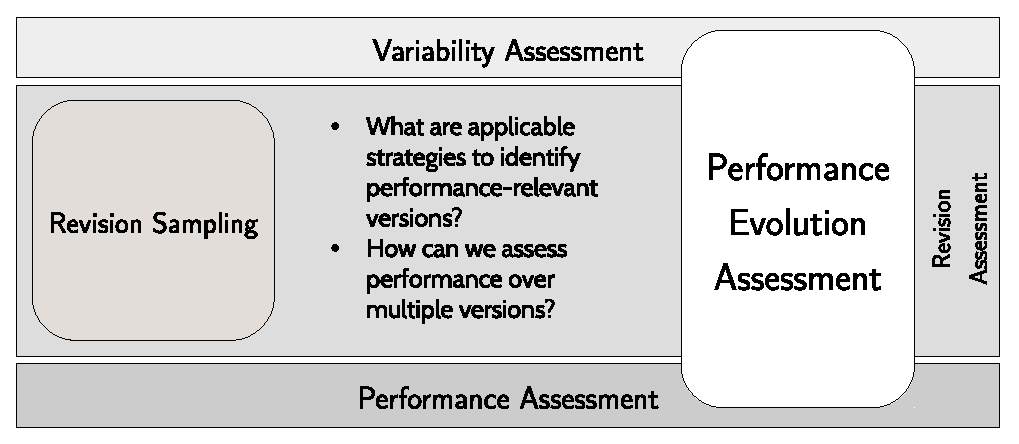
\includegraphics[width=0.75\textwidth]{images/process_revassesment.eps}
	\caption{Methodological road-map: questions to address with revision
	assessment.}
	\label{fig:roadmap_2}
\end{figure}

The chapter is organized as follows. In section~\ref{sec:towards_revsampling} we
present the methodological requirements for a designing and selecting a revision sampling
strategy. In section ~\ref{sec:revsampling_strat} we propose four approaches to
revision sampling based on observations of configurable software systems. In
section~\ref{sec:revsampling_eval} we evaluate the different approaches against
exhaustive measurements of a selection of configurable software systems.
Finally, in section~\ref{sec:revsampling_method} we conclude the chapter and
discuss the approaches' applicability in the context of our methodology.

\section{Towards Revision Sampling}\label{sec:towards_revsampling}
Research so far has addressed the assessment of a software system’s revision
history under the umbrella of repository mining, for instance, to localize bugs
\citep{moin_bug_2010} or performance regression \citep{heger_automated_2013}.
Nonetheless, so far there exists little to no research addressing the question
what the choice of versions might reveal about performance evolution. The task
of selecting resources and a sample set of versions to analyze can be conceived
as a sampling strategy, where the objective is to cover interesting entities
(performance changes, in our case) while trying to limit the sample size to
keep the required effort reasonable. Before we present different approaches to
select a sample set of revisions, we need to define general cornerstones for
evaluating a sample set of revisions as well as respective revision sampling
strategies with respect to performance change history.

\paragraph{Revision Sample Set.} The first question is, what criteria we take as
a basis for rating a sample set of revisions as \emph{meaningful}. First, our intention
is to obtain a representative description of a software system’s performance
change history while only assessing a fraction of revisions. That is, assessing
a representative sample of revisions should yield a performance change history
similar to the assessment of all revisions. Since we are interested in
revisions for which performance measurements change, these revisions should be
contained in a representative sample. Second, especially in the context of
variability, a performance change might only affect a subset of the assessed
configurations. A representative sample set, therefore, should describe a
history of significant performance changes with respect to all variants
assessed. We consider a performance change to be significant, if it affects a
significant portion of the sample of variants (\emph{effect range}) and if the
relative change in performance measurements is significantly large (\emph{effect
magnitude}).

\begin{figure}[h!]
	\centering
	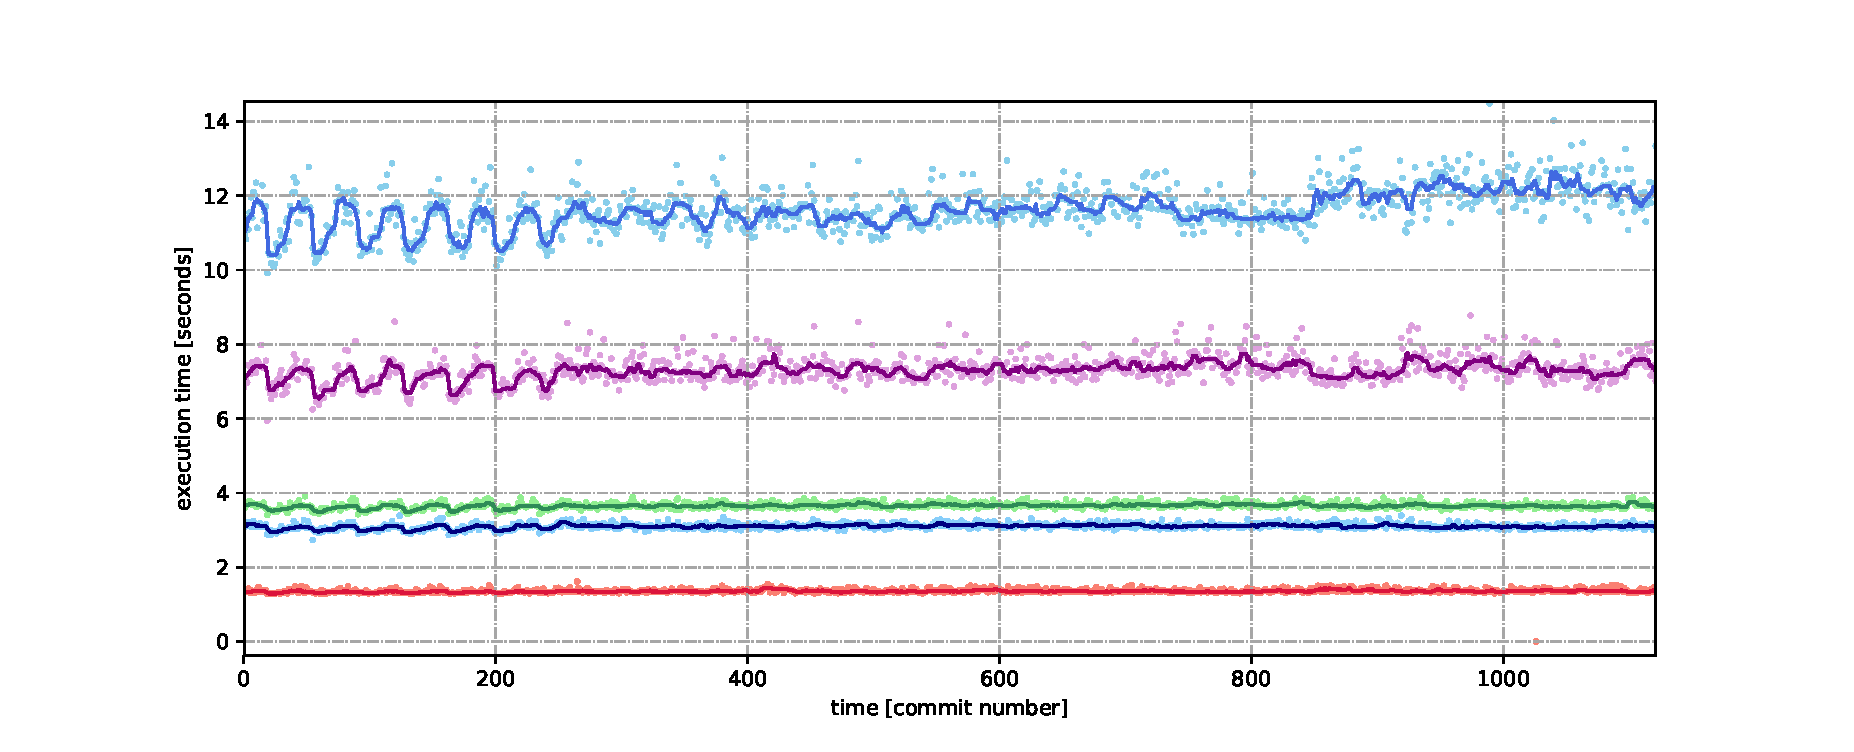
\includegraphics[width=0.95\textwidth]{images/xz_sample_evolution.eps}
	\caption{Performance History for XZ}
	\label{fig:xz_evosample}
\end{figure}

To illustrate the two facets of performance changes, in
Figure~\ref{fig:xz_evosample} we see a history of performance measurements (execution time in this case) for a
small-scale configurable software system, file compression tool called \emph{GNU
XZ Utils}. The graphic depicts execution time measures for executing a standard
compression benchmark for $1,135$ different versions and covers a version
history of about nine years. In this excerpt, we only show the execution time measures
of four different variants, i.e., each version was assessed with four different
configurations. One can see that the execution time for the red and the green
configurations remains stable and does not fluctuate, while for the blue and
grey configuration, the execution time measures are generally more volatile.
Moreover, between 2010 and 2012, performance for the latter variants fluctuates
heavily. With regard to the two facets of significance mentioned above, not all
variants are affected similarly by this effect. That is, if performance were
assessed solely for one of the non-fluctuating variants, no performance
evolution could be identified.

While the former significance criterion can unambiguously defined by a threshold
number of variants, for the latter one one needs to define how to summarize
relative performance change among all variants. For instance, a performance
change may have a significant magnitude, if the average deviation of
performance measurements for all variants is greater than a specified threshold
value.

\paragraph{Revision Sampling Strategies.} The second question addresses the
rationale behind a revision sampling strategy. To obtain representative sample sets, sampling
strategies are intended to utilize knowledge about the total volume to select
sample sets from. For instance, pair-wise sampling aims to cover most feature
interactions. Similarly, we demand for a meaningful revision sampling strategy
to exhibit a certain rationale or coverage criterion. If we conceive a sampling
strategy as a binary classificator that, in our case, decides whether in a
revision a performance change is likely, or performance measurements might have
changed compared to prior commits, we want  this classifier to be sensitive,
i.e., to have a preferably high true positive rate. That is, a sampling
strategy is meaningful if we learn which revision features most likely indicate
performance changes.\\

In conclusion, when designing a revision sampling strategy, we ask for a
plausible rationale or coverage criterion with respect to performance changes.
A resulting sample set of revisions, in addition, is representative, if the
contained revisions sketch performance changes. For the context of this
methodology, we remain with a clear definition of what performance
changes are significant. Based on these assumptions, in the next section we
propose a selection of four revision sampling approaches based on different
observations.
 
\section{Revision Sampling Strategies}\label{sec:revsampling_strat}

\begin{figure}[h!]
\centering
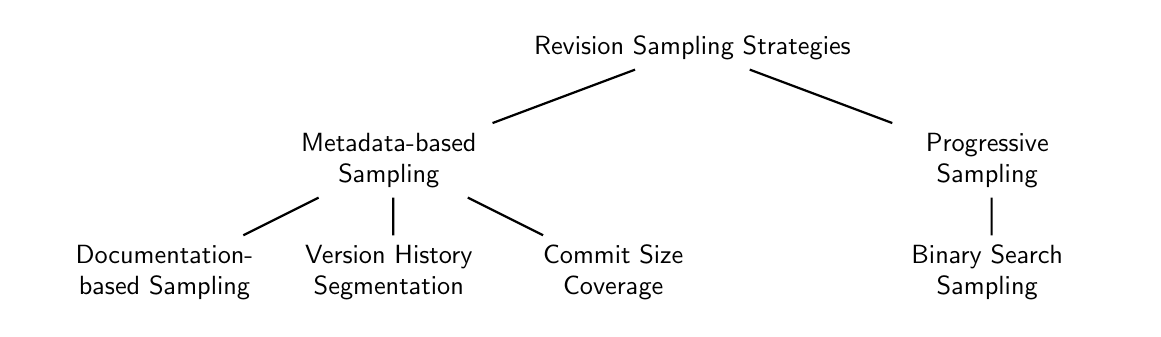
\begin{tikzpicture}[%sibling distance=15em,
level 1/.style={sibling distance=8cm},
level 2/.style={sibling distance=3cm}, 
level 3/.style={sibling distance=6cm},
  every node/.style = {rounded corners,
    draw, align=center,
    top color=white, bottom color=blue!20},thick,scale=0.95, every
    node/.style={scale=0.95}]
  \node {\sffamily Revision Sampling Strategies}
    child { 
    	node [align=left] {
    		\begin{tabular}{c} 
    			{\sffamily \parbox{3cm}{\centering Metadata-based Sampling}}
    		\end{tabular}
    	}
    	child { 
    		node [align=left] {
    			\begin{tabular}{c}
    				{\sffamily \parbox{3cm}{\centering Documentation-based Sampling}}
    			\end{tabular}
    		}
    	} 
    	child { 
    		node [align=left] {
    			\begin{tabular}{c} 
    				{\sffamily \parbox{3cm}{\centering Version History Segmentation}}
    			\end{tabular}
    		}
    	}
    	child { 
    		node [align=left] {
    			\begin{tabular}{c} 
    				{\sffamily \parbox{3cm}{\centering Commit Size Coverage}}
    			\end{tabular}
    		}
    	} 
    }
    child { 
    	node [align=left] {
    		\begin{tabular}{c} 
    			{\sffamily \parbox{3cm}{\centering Progressive Sampling}}
    		\end{tabular}
    	} 
    	child { 
    		node [align=left] {
    			\begin{tabular}{c}
    				{\sffamily \parbox{3cm}{\centering Binary Search Sampling}}
    			\end{tabular}
    		}
    	}
    	};
%    	child { 
%   		node [align=left] {
%	    		\begin{tabular}{c} 
%	    			{\sffamily \parbox{3cm}{\centering Hot-Spot Sampling}}
%	    		\end{tabular}
%    		}
%    	} 
%    };
\end{tikzpicture}

\caption{Overview of our proposed revision
sampling strategies.}\label{fig:revsampling_overview}
\end{figure}

\subsection{Documentation-driven Sampling}
\subsection{Version History Segmentation}
\begin{figure}[h!]
\def\tabularxcolumn#1{m{#1}}
\begin{tabularx}{\linewidth}{@{}cXX@{}}
\centering
\begin{tabular}{cc}
\subfloat[Activity graph for \texttt{GNU XZ}, generated from 1,135 versions
between December 8, 2007, and August 14, 2017.]
{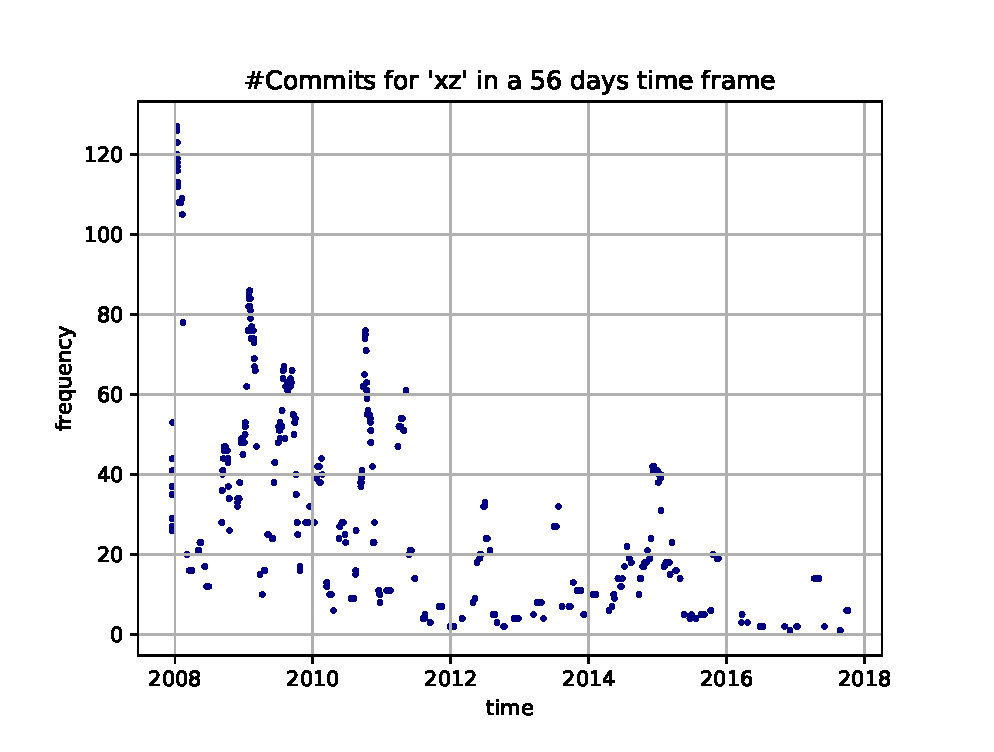
\includegraphics[width=0.45\textwidth]{images/activity_xz.eps}}
&
\subfloat[Activity graph for \texttt{x264}, generated from 2,851 versions
between June 3, 2004, and June 26, 2017.]{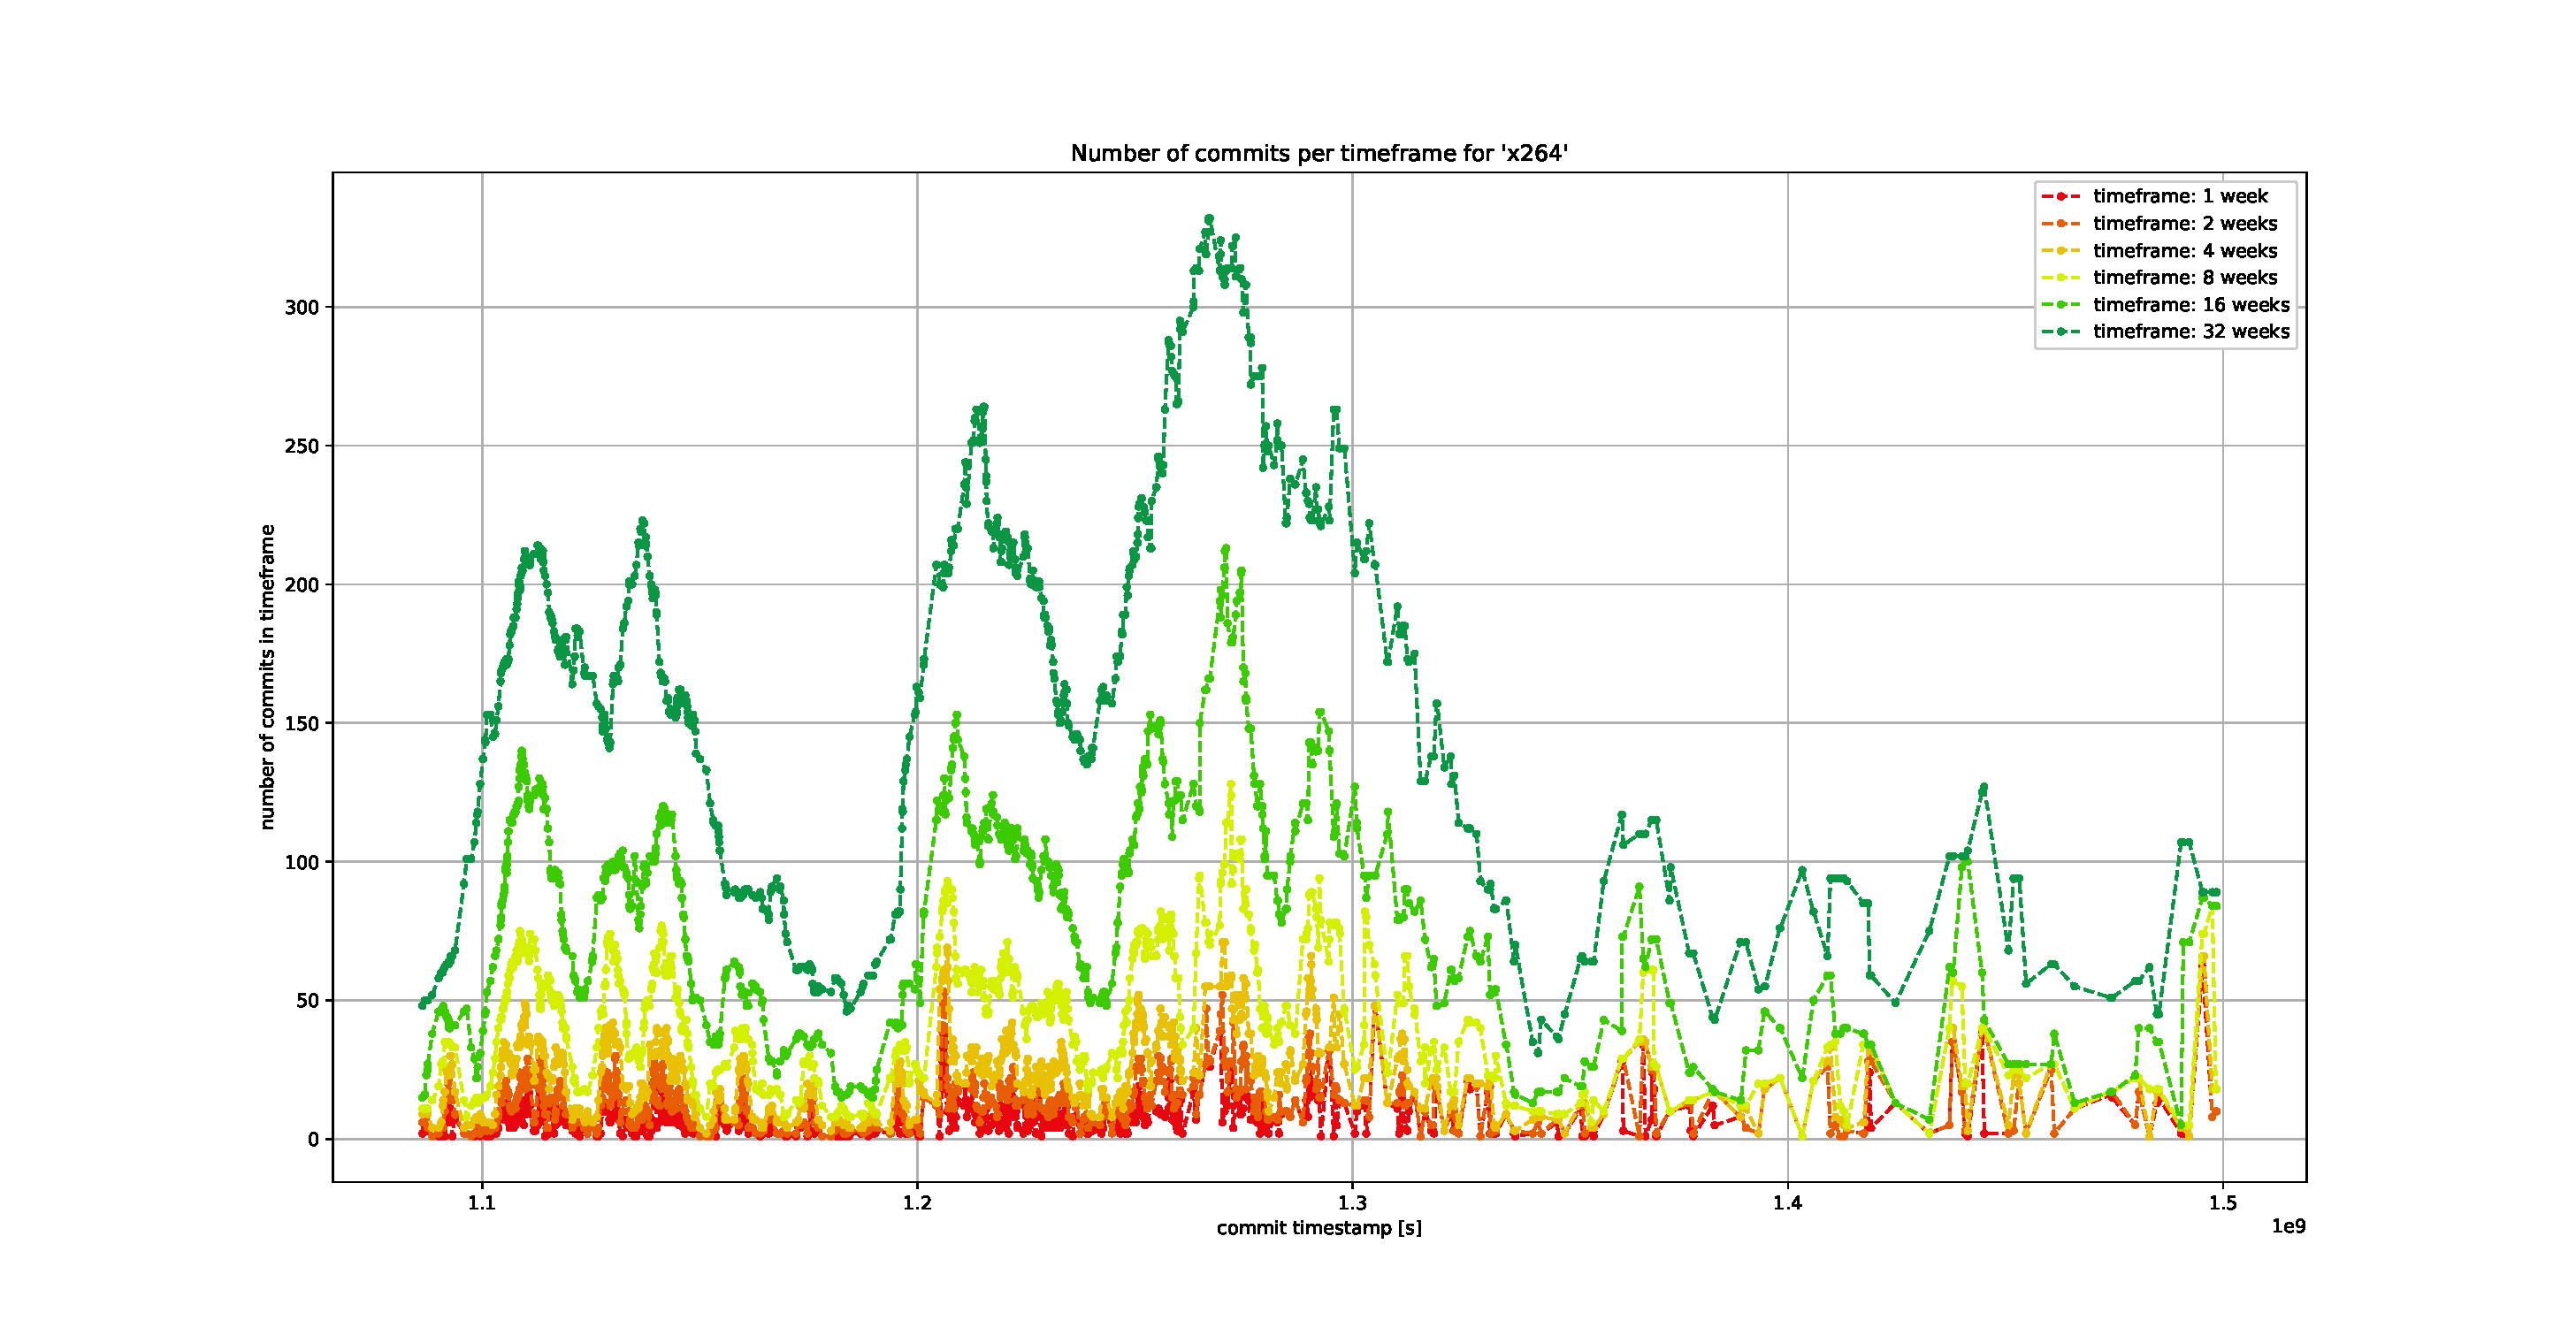
\includegraphics[width=0.45\textwidth]{images/activity_x264.eps}}\\
\end{tabular}
\end{tabularx}
\caption{Commit activity for two sample systems, the compression
utility \texttt{GNU XZ} and the video encoder \texttt{x264}. For each version,
the activity is measured as the number of commits that were pushed within a
certain timeframe of eight weeks.}
\label{fig:ActivityGraphs}
\end{figure}

\begin{figure}[h!]
\def\tabularxcolumn#1{m{#1}}
\begin{tabularx}{\linewidth}{@{}cXX@{}}
\centering
\begin{tabular}{cc}
\subfloat[Distribution of time to next commits for \texttt{GNU XZ}]
{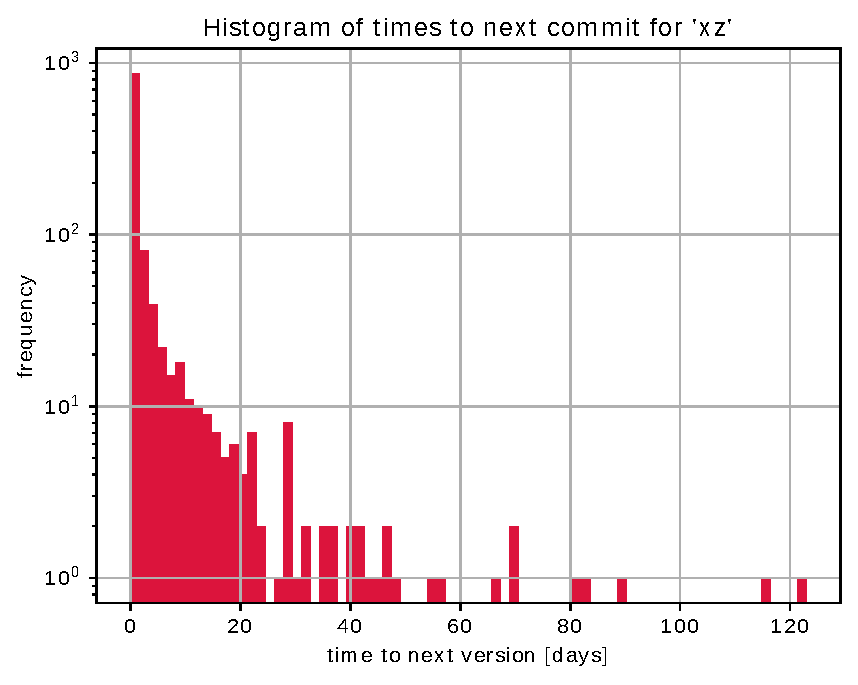
\includegraphics[width=0.45\textwidth]{images/commit_differences_xz.eps}}
&
\subfloat[Distribution of time to next commits for \texttt{x264}]
{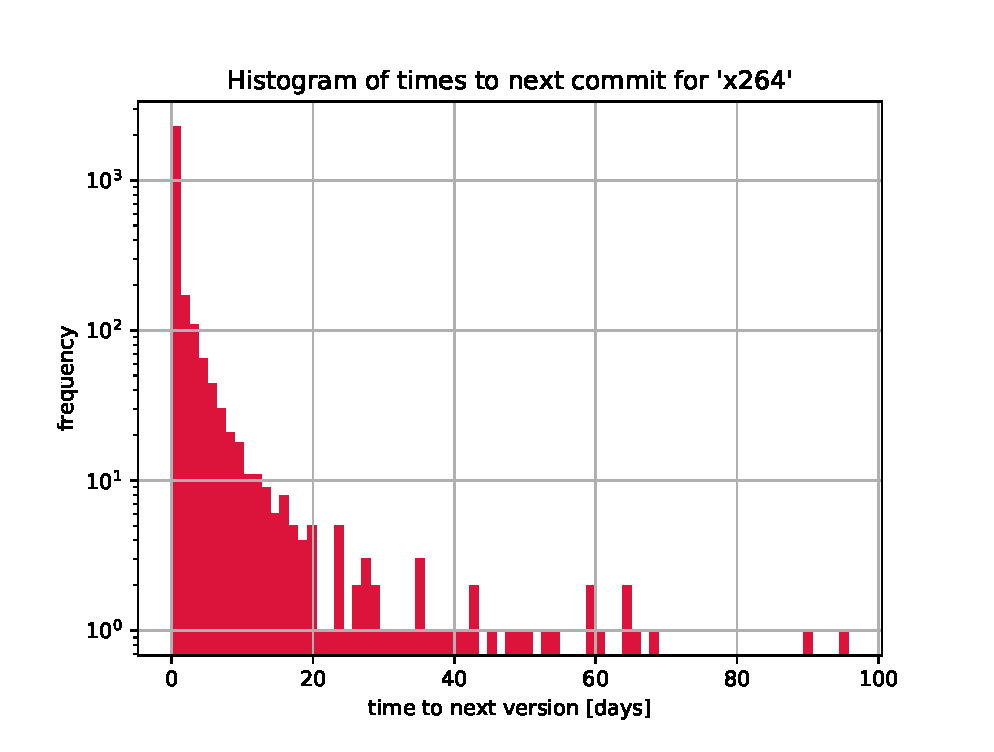
\includegraphics[width=0.45\textwidth]{images/commit_differences_x264.eps}}\\
\end{tabular}
\end{tabularx}
\caption{Distribution of time to next commits for two configurable software
systems, measured as the distance between a commit and its successor.}
\label{fig:bener}
\end{figure}

\subsection{Change Coverage Sampling}
\begin{figure}[h!]
\def\tabularxcolumn#1{m{#1}}
\begin{tabularx}{\linewidth}{@{}cXX@{}}
\centering
\begin{tabular}{cc}
\subfloat[Distribution of changed lines per commit for \texttt{GNU XZ}]
{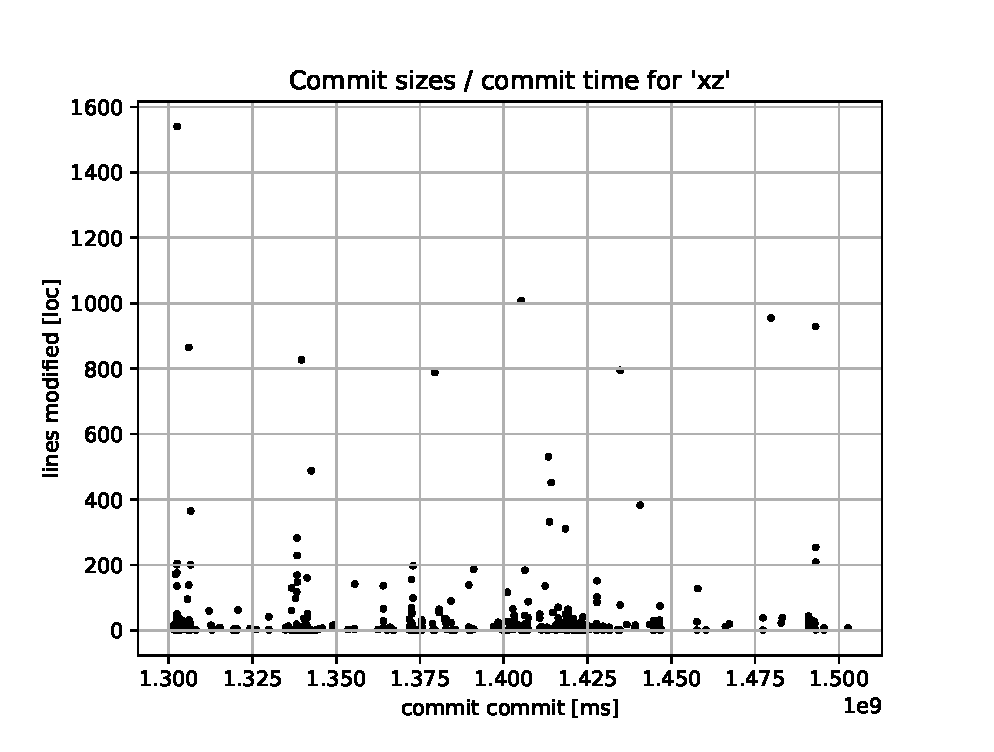
\includegraphics[width=0.45\textwidth]{images/commit_sizes_xz.eps}}
&
\subfloat[Distribution of changed lines per commit for \texttt{x264}]{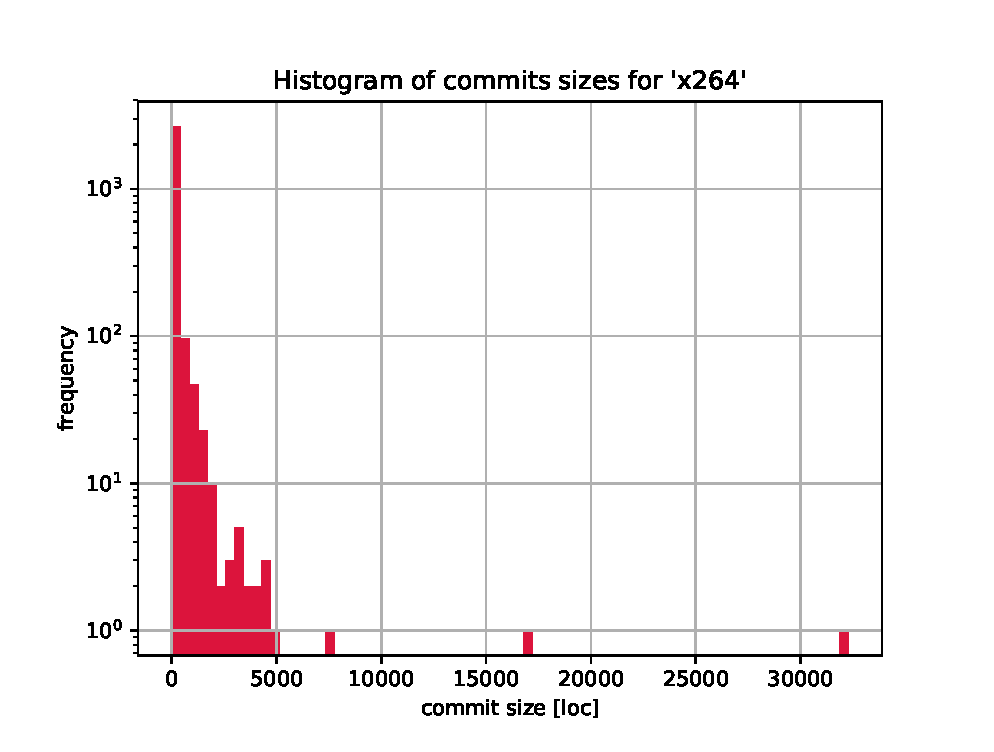
\includegraphics[width=0.45\textwidth]{images/commit_sizes_x264.eps}}\\
\end{tabular}
\end{tabularx}
\caption{Distribution of commit sizes in lines of code for two configurable
software systems, \texttt{GNU XZ} and \texttt{x264}.}
\label{fig:bener}
\end{figure}
\subsection{Binary-Search-based Sampling}
\subsection{Hot-Spot Sampling}

\section{Strategy Evaluation}\label{sec:revsampling_eval}
\section{Methodological Remarks}\label{sec:revsampling_method}

%\begin{figure}
%\def\tabularxcolumn#1{m{#1}}
%\begin{tabularx}{\linewidth}{@{}cXX@{}}
%\begin{tabular}{c}
%\subfloat[Activity Graph for \texttt{GNU XZ}, generated from 399 versions
%between March 24, 2017, and August 14, 2017. The earliest release version is
%\texttt{5.1.1alpha}, the latest is \texttt{5.3.0alpha}.]
%{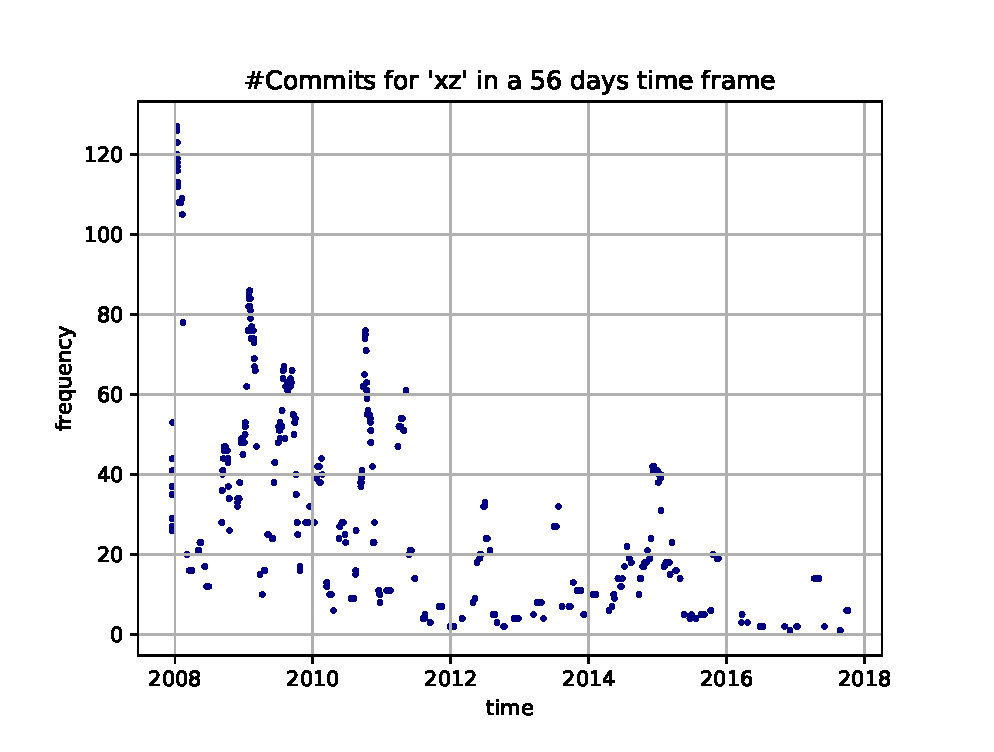
\includegraphics[width=0.99\textwidth]{images/activity_xz.eps}}
%\\
%\subfloat[Activity Graph for \texttt{x264}, generated from 2851 versions
%between June 3, 2004, and June 26, 2017. The earliest release version is
%\texttt{BUILD 1} from, the latest is \texttt{BUILD 149} from
%X.]{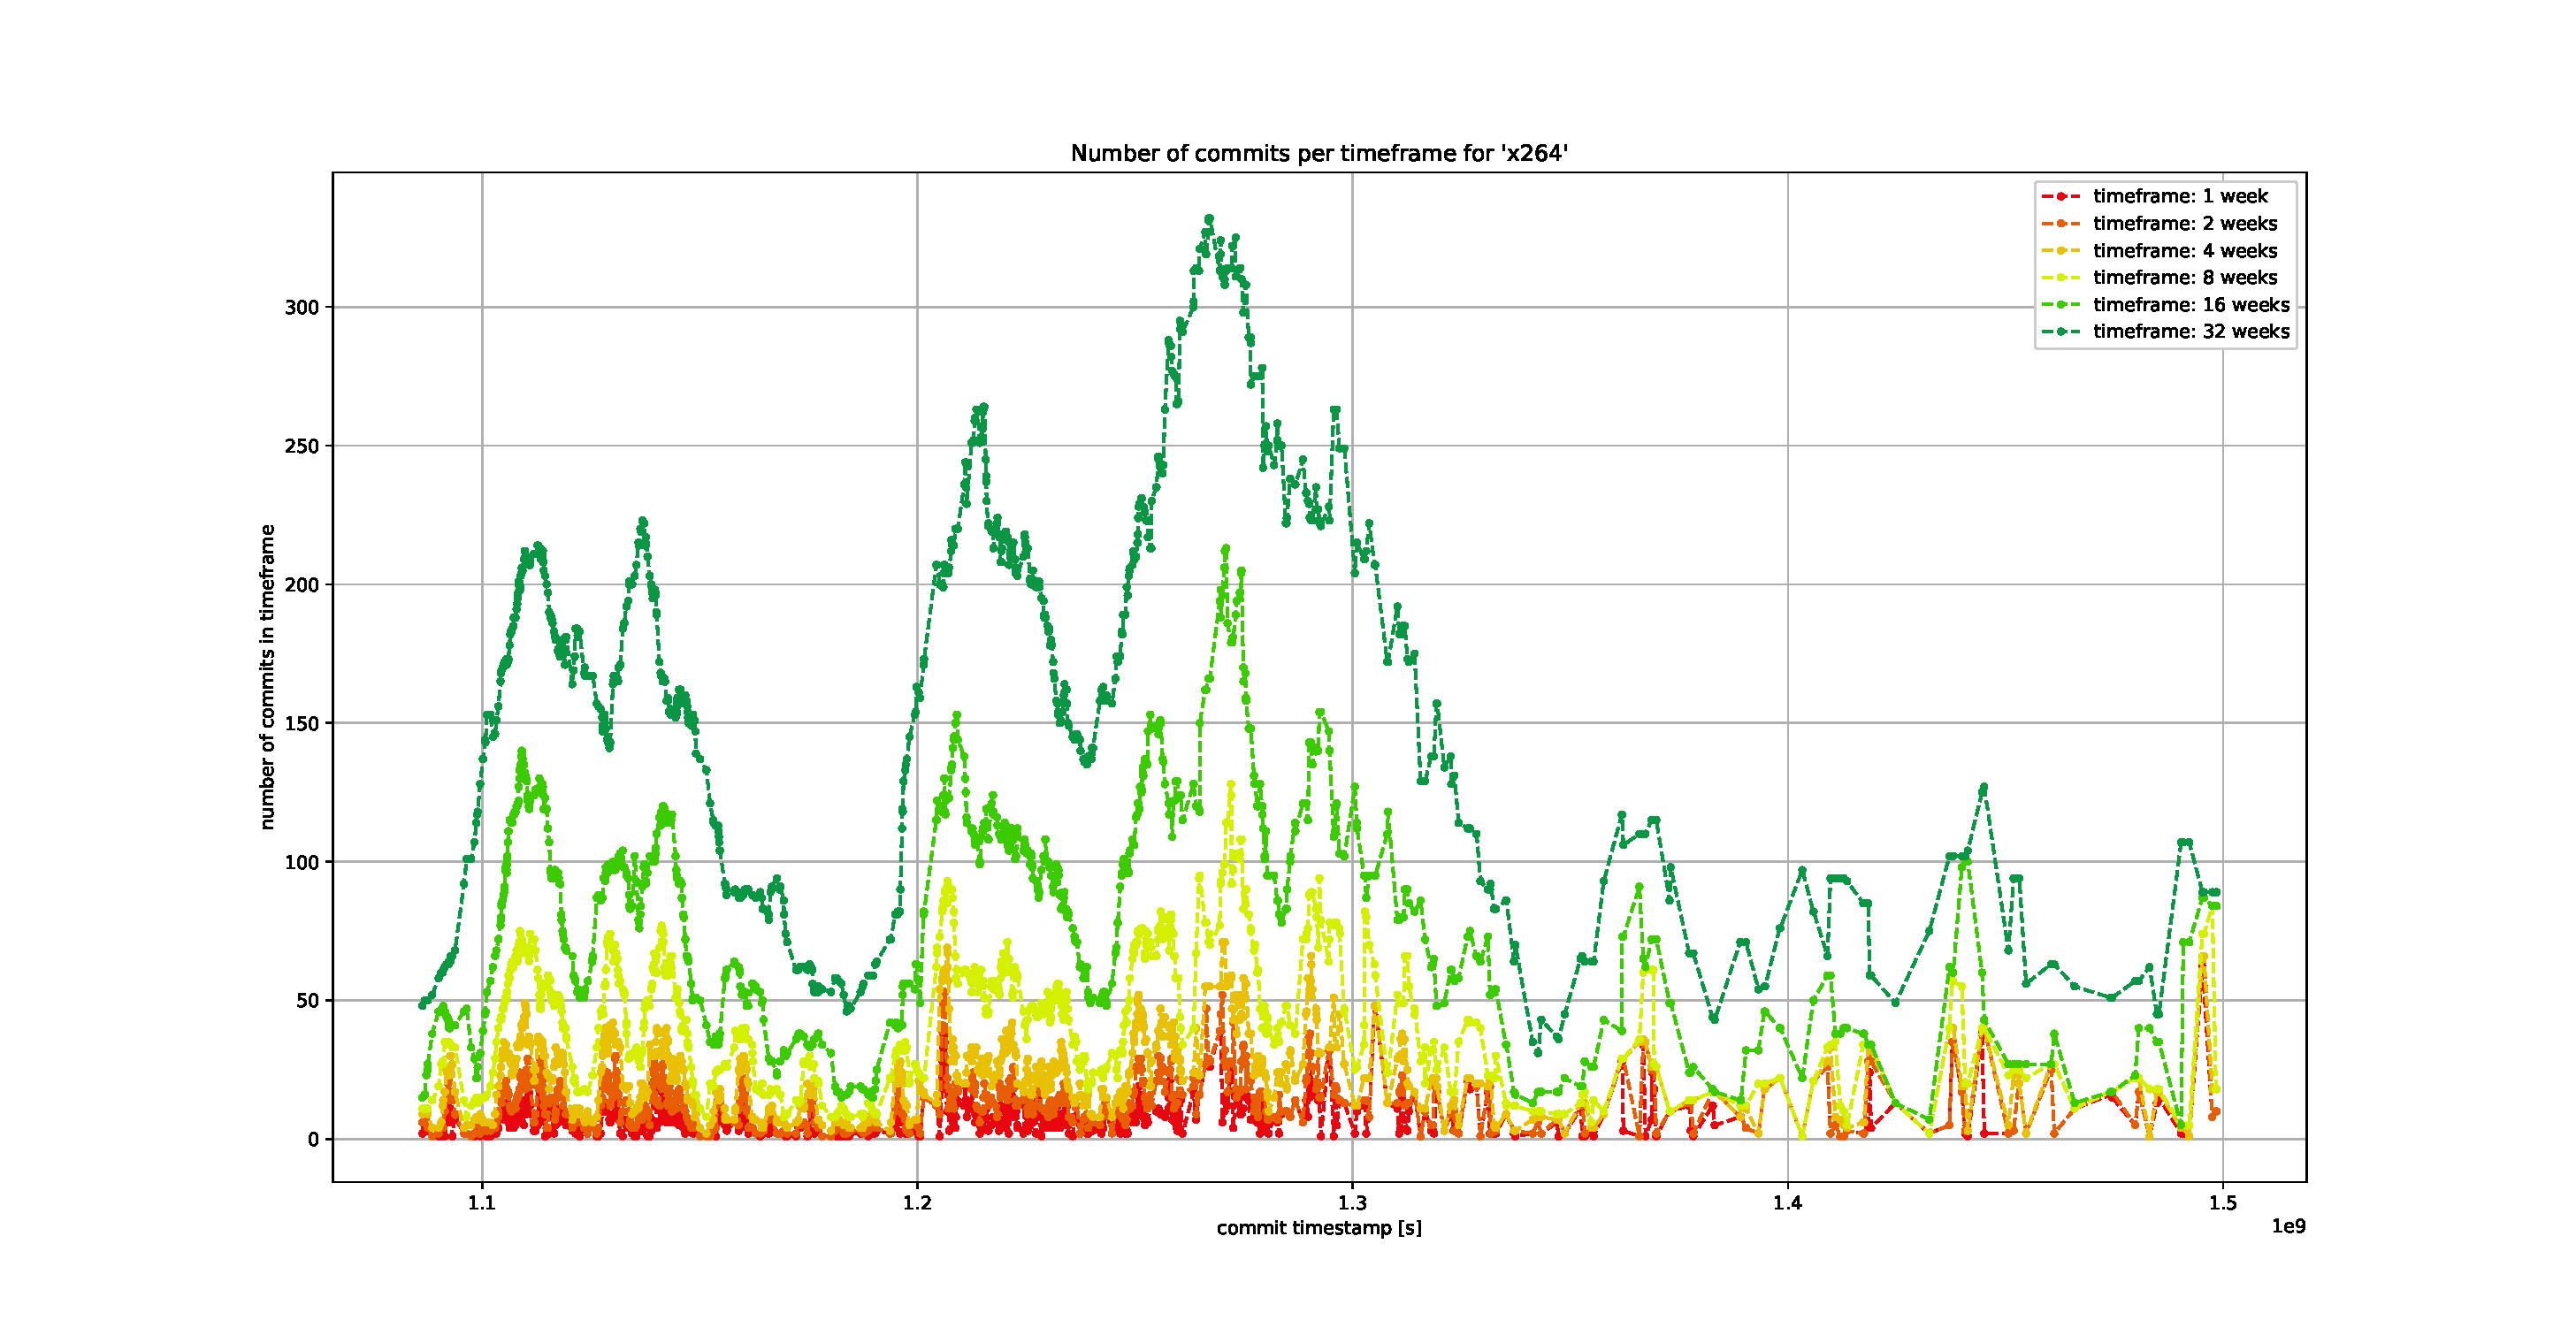
\includegraphics[width=0.99\textwidth]{images/activity_x264.eps}}\\
%\end{tabular}
%\end{tabularx}
%\caption{Commit activity for two sample systems, the compression
%utility \texttt{GNU XZ} and the video encoder \texttt{x264}. For each version,
%the activity is measured as the number of commits that were pushed within a
%certain timeframe after or before the actual commit. The timeframes range from
%one week to 32 weeks, as shown in the legendary.}
%\label{fig:ActivityGraphs}
%\end{figure}


\chapter{Methodology: Performance Assessment}\label{chapter:5}
The last two chapters covered methodological guidelines for variability as well
as version assessment. While those two terms, \emph{variability} and
\emph{versions} represent two orthogonal dimensions of a configurable software
systems’ evolution history. To provide a closed description of guidelines for performance
evolution assessment, this chapter finally presents a guideline to assessing
performance for a given variant and version. In Figure~\ref{fig:roadmap_3}, we
present the methodological roadmap and questions to be answered in this chapter.

\begin{figure}[h!]
	\centering
	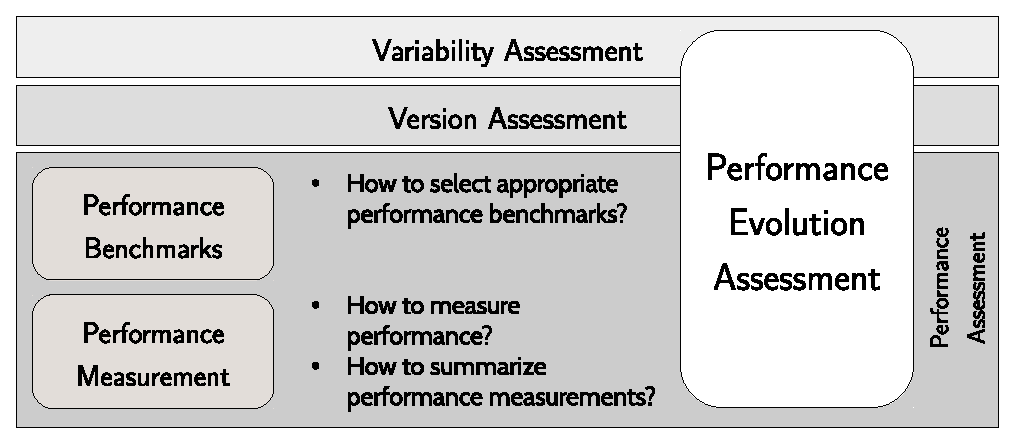
\includegraphics[width=0.99\textwidth]{images/process_perfassessment.eps}
	\caption{Methodological road-map: performance assessment}
	\label{fig:roadmap_3}
\end{figure}

First, in section we categorize software systems with respect to the availability of suitable performance
benchmarks; second, we outline the general properties of profiling tool support
used throughout dynamic program analysis; finally, we discuss different statistical
with respect to their applicability in the context of performance assessment
and robustness.

\section{Performance Benchmarks}
The essential part of assessing performance for a software system is the choice
of a benchmark that one wants to evaluate the software against. For the choice
of a suitable benchmark, two consecutive questions need to be answered. First of
all, we need to specify, what aspects of performance we intend to evaluate for
our software system. As presented earlier in chapter\,\ref{chapter:2}, the term
\emph{performance} is generic as it is commonly outlined by different key
performance indicators. For instance, for a web shop application, good performance is characterized by low response
time and high availability, while for file compression, one might rather
conceive high throughput as good performance. That is, given a specific
aspect of performance, i.e., one or more KPIs, for a software system, from
testing against a suitable performance benchmark one needs to be able to judge
whether the specified performance goals are met or not.

Next, once we have specified performance indicators fitting our software system,
we need to select a benchmark, i.e., a repeatable task for the software system
for which we can evaluate performance. To keep performance measurements
comparable throughout all versions and variants, it is required to use
only one benchmark per assessment. Following this principle, and to even compare different software
systems, practitioners are advised to refer to reusable, or more general
performance benchmarks whenever possible. To illustrate this, we can divide
software systems into three general categories for which we are presenting
separate strategies.

First, in the the easiest case, a software system provides software tests, or
performance benchmarks, to use for performance assessment. The idea of using an
existing test suite to assess performance is straightforward and has already
been applied to detect performance regression
\citep{foo_mining_2010,heger_automated_2013}.

Second, a software system can offer functionality for a domain, where
standardized benchmarks have been established, or are commonly used to compare
performance measurements. For instance, for the domain of file compression
there exists a long tradition of using standardized file sets as performance
benchmarks, such as the Canterbury
or Calgary corpus\footnote{See
\url{http://corpus.canterbury.ac.nz/descriptions/} for a detailed 
description.}; for video encoding, the
xiph.org\footnote{\url{https://media.xiph.org/}} foundation provides a large set of video benchmark files; and, more general, for processors the Standard
Performance Evaluation Corporation provides (SPEC) standardized benchmarks for
floating point operations. Whenever a software system falls under a domain for
which standardized benchmarks exist, we advocate to use those.

Finally, if neither a performance benchmark or test suite is available for a
software system, nor domain-specific benchmarks exist, the task of designing a
benchmark is left to the practitioner evaluating the software. As the
conception of performance is generic and highly context-dependent, there is no
standardized recipe for designing a performance benchmark. However, the main
criteria to be satisfied include \emph{expressiveness}, \emph{cost-efficiency}
and \emph{reproducibility}. First, a suitable performance benchmark should
clearly express what a desirable and unfavorable performance measurement is, given a specified
key performance indicator. For instance, if we evaluate performance in terms of
response, or execution time, minimal measurements are desirable. Second, effort
that is required to evaluate a software with a benchmark must be reasonable.
Since performance measurements are usually repeated to decrease measurement
bias, or used for different variants and revisions, performance benchmarks
should be limited in terms of size. However, a performance benchmark needs to
be large enough to sketch performance changes or deviations. Finally, the
construction of a benchmark must be reproducible, i.e., transparent and
plausibly designed as the overall value of a performance benchmark depends on
whether we can draw any conclusion from performance measurements obtained from
it.

In conclusion, for the context of our methodology, the advocated guideline for
selecting and designing a performance benchmark for a configurable software
system is to select a benchmark as generic as possible. If there is no reusable
benchmark available, the design of any performance benchmark should follow the
criteria of expressiveness, cost-efficiency, and reproducibility.

\section{Profiling}
With a software system along with a benchmark set up, the only choice left
before assessing performance is to select a means to obtain and collect
performance measurements. For this type of tool support for dynamic analysis,
commonly referred to as profilers, exists a variety of solutions, varying in
functionality and scope of application.

\cite{satapathy_survey_2015} have surveyed a selection of profilers for dynamic
analysis. The authors categorize their selection into three categories,
including VM-profiling-based, instumentation-based, and profilers based on
aspect-oriented programming (AOP). While for VM-based profilers, make use of
profiling functionality offered by the respective platform, such as the Common
Language Interface (CLI) for the family of .NET languages,  or the Java Virtual
Machine (JVM), instrumentation-based profilers add instructions to the software
to the software’s codebase at compilation using instrumentation preprocessors,
or to the software’s executables. AOP-based profilers accommodate profiling
functionality in separate modules called aspects. An aspect’s code, called
advise is executed whenever a corresponding event, called join point,  occurs,
for instance a call of a function that one would like to measure performance
for. Several join points can be summarized by a set of join points, called
point cut. While VM-based profilers are limited to a family of programming
languages, and, as well as instrumentation-based, usually introduce a run-time
overhead that might dilute performance measurements. In contrast to that,
AOP-based profilers  usually perform better, yet are limited to the code base as aspects
are woven into the codebase during re-compilation. Moreover, they require a
higher level of expertise to design and deploy a performance test setup
compared to the former two categories \citep{satapathy_survey_2015}. In addition
to the aforementioned profiler categories, statistical profilers such as
\emph{Performance Counters for
Linux}\footnote{See
\url{http://man7.org/linux/man-pages/man1/perf-stat.1.html} for further
information on \texttt{perf}.}, or \emph{perf}, monitor a software system
performance, for instance hardware counters for regular intervals, and therefore provide an approximation of the software system’s performance with less overhead than instrumentation-based profilers.

In the context of our methodology, we are advocating the use of the unix
command \texttt{time}\footnote{See
\url{http://man7.org/linux/man-pages/man1/time.1.html} for the man page of
\texttt{time} and provided performance metrics to record.} to measure execution
time along with a number of further performance metrics for a software system.
The command is contained in most Linux distributions and, from a black-box
perspective, provides sufficient functionality to sketch performance in terms of
metrics for execution time, memory consumption, or I/O statistics. While tools falling under the aforementioned categories are powerful tools for dynamic analysis and program
optimization, \texttt{time} provides a basic, yet exhaustive support for
assessing performance for software system run on a single host machine. 

\section{Statistical Considerations}\label{sec:statistical_considerations}
In this section, we now discuss the appropriate statistical means to summarize,
compare and interpret measurement results. For the remainder of this section, we
will refer to the following two scenarios. First, to obtain robust results, the
assessment of a single variant needs to be repeated multiple times.
Consequently, to report a single result per metric, the measurements for a
single variant need to be summarized. Second, the assessment of performance for
a variant may comprise several use cases, for instance file
compression and decompression for a compression software. Therefore, performance measures
aggregated from different benchmarks need to be summarized accurately. 

\subsection{Measures of Central Tendency}
For each test run of a software system or variant, we obtain a single-valued
measurement per performance metric. Since we repeat each test run $n$ times
per variant, we obtain a data record $X$ with $n$ measurements $X = X_1, X_2,
\ldots, X_{n-1}, X_n$. While the arithmetic mean is commonly considered the
right way to summarize data records and report a representative average
value, we need to be more cautious with how to summarize data records
\citep{fleming_how_1986,smith_characterizing_1988}. From a statistical
perspective, the intention of summarizing a data record is to find a measure of
central tendency what is representative for the data record.
While the arithmetic mean is an appropriate method for many cases, there exist
other means to summarize data records. Moreover, there exist a number of
criteria for when to use which means to summarize a data record. 

The first question when summarizing a data
record is to ask what the data actually describe and what we intend to express
with our summary. For a data record $X$, we can define a
relationship we would like to conserve while replacing each single $X_i$ with an
average value $\bar{x}$. Based on this relationship, we can derive the
appropriate method to summarize our record. For instance, our data record $X$
describes the time elapsed for a test case and we want the keep the following
relation, saying that the sum of all measurements $\sum_{i = 1}^{n} X_i$ is
equal to the total time elapsed $T$, defined as

$$
T = \sum_{i = 1}^{n} X_i = \sum_{i = 1}^{n} \bar{x}.
$$

Based on the term above, we can derive the definition of the method
appropriate to summarize our data record with respect to the conserved relation
what is the \emph{arithmetic mean}, defined as

\begin{equation} \label{eq:arithmetic_mean}
\begin{split}
\bar{x} = \frac{1}{n} \sum_{i = 1}^{n} X_i.
\end{split}
\end{equation}

Consider another example, similar to the one above, where the test
case is a load test with a predefined number of users and the measurements $X =
X_1, X_2, \ldots, X_{n-1}, X_n$ are
measured as hits per second. Again, we have different measurements we want to
summarize with respect to a relation to conserve. Each user drops the same
number of requests $T$, whereby the hit rate $X_i$ and the respective elapsed
time $t_i = \frac{T}{X_i }$ vary. We now conserve the relationship that the
total number of requests for the data record is the sum of all hit rates $X_i$
times the time elapsed $t_i$. Therefore, we want to substitute each hit rate
$X_i$ with an average value $\hat{x}$ so that the aforementioned relationship is
conserved:

$$
n\cdot T - \sum_{n}^{i=1} X_it_i = 0 \Leftrightarrow n\cdot T - \hat{v}
\sum_{n}^{i=1} t_i = 0 \Leftrightarrow n = \hat{x} \sum_{n}^{i=1} \frac{1}{X_i}
$$

Similar to Eq. \ref{eq:arithmetic_mean} we can derive the definition for the summarization
method to use from the equation above what is the \emph{harmonic mean}, defined as

\begin{equation} \label{eq:harmonic_mean}
\begin{split}
\hat{x} = n \cdot \bigg(\sum_{i=1}^{n} \frac{1}{X_i}\bigg)^{-1} =
\frac{n}{\frac{1}{X_1} + \frac{1}{X_2} + \ldots +
\frac{1}{X_{n-1}} + \frac{1}{X_n}}.
\end{split}
\end{equation}

We see that the summarization methods presented in Eq. \ref{eq:arithmetic_mean}
and \ref{eq:harmonic_mean} are useful for different types of data records, and
should be used accordingly. The arithmetic mean is suitable for records, where the total sum of single
measurements has a meaning, whereas the harmonic mean is suitable for measured
rates or frequencies \citep{smith_characterizing_1988}.

While the aforementioned measures of central tendency should be appropriate for
most cases, they are not always the best choice though since the arithmetic
and harmonic mean are heavily influenced by extreme observations
\citep{shanmugam_statistics_2015}. 
For instance, for the data record $X = 1, 2, 3, 30$, three of four values are
smaller than the arithmetic mean $\bar{x} = 9$. One option is to explicitly exclude outlier
values from the data record. The so-called \emph{trimmed mean} is
obtained by truncating a upper and/or lower percentage $t$ of the data record
and, consequently, computing the (arithmetic or harmonic) mean for the remaining
data record \citep{shanmugam_statistics_2015}. 

While this method is suitable to omit the effects of outliers, one still needs to specify
which upper and/or lower percentage $t$ needs to be truncated. Moreover, the use
a (trimmed) mean requires the data records' frequencies to be distributed
symmetrically around its mean.
A probability distribution is skewed (and therefore asymmetric) if, graphically speaking, its histogram is not
symmetric around its measure of central tendency. A simple method to measure the
skewness of a probability distribution is \emph{Bowley's measure}
\citep{shanmugam_statistics_2015}, defined as

\begin{equation} \label{eq:bowley}
\begin{split}
B_S = \frac{(Q_3 - M) - (M - Q_1)}{Q_3 - Q_1} = \frac{(Q_3 + Q_1 - 2M)}{Q_3
- Q_1},
\end{split}
\end{equation}

where $Q_1$ and $Q_3$ denote the first and third quartile, and $M$ denotes the
median of the probability distribution. The quartiles $Q_i$ with $i \in \left\{
1,2,3 \right\}$ are defined as the values of a data record $X$, so that
$\frac{i}{4}$ of the values of $X$ are smaller than $Q_i$. The \emph{median} is
defined as $Q_2$, i.e., a value $M \in X$ so that half of the values in $X$ are smaller than $M$.

The median itself is a more robust measure of central tendency than the
aforementioned ones since it is less influenced by outliers and can be used for
both skewed and symmetric data records \citep{shanmugam_statistics_2015}. For a
given ascendingly ordered data record $X = X_1, X_2, \ldots, X_{n-1}, X_n$, we
can compute the median as follows:

\begin{equation} \label{eq:median}
\mathrm{Median}(X) = \begin{cases}
     X_{\frac{n+1}{2}} & \text{if $n$ is odd} \\
     \frac{1}{2}\big(X_{\frac{n}{2}} + X_{\frac{n}{2}+1}\big) & \text{if $n$ is
     even}
   \end{cases}~\text{with $X_i \leq X_j$ and $i < j \leq n$ }
\end{equation}

\subsection{Measures of Dispersion}

Last, we take a look at different measures of spread or dispersion. Most
commonly used are the \emph{variance} $\sigma^2$ and the \emph{standard
deviation} $\sigma = \sqrt{\sigma^2}$ defined along the mean $\mu$ of a
probability distribution as

\begin{equation} \label{eq:variance}
\begin{split}
\sigma^2 = \frac{\sum_{i=1}^{n}(X_i - \mu)^2}{n}
\end{split}
\end{equation}

Similar to the (arithmetic or harmonic) mean, the variance and the standard
deviation are heavily influenced by extreme observations
\citep{shanmugam_statistics_2015} and not the best choice in all cases. Instead,
two more robust measures are the \emph{median absolute deviation} (MAD) and the \emph{inter-quartile range} (IQR). The MAD is defined as the median of the absolute deviations from the probability distributions'
median \citep{molyneaux_art_2014}, or, defined as follows:

\begin{equation} \label{eq:mad}
\begin{split}
\mathrm{MAD}(X) = \mathrm{Median}\big(|X - \mathrm{Median}(X)|\big)
\end{split}
\end{equation}
 
The IQR, however, defines the range between the first and the third quartile,
$Q_1$ and $Q_3$ \citep{shanmugam_statistics_2015}. This range is larger for a
widespread data record and smaller for a data range with a narrow spread, but is not influenced by extreme
observations as those outliers do not lie within the range $\left[ Q_1,Q_3
\right] $. The IQR is defined as 

\begin{equation} \label{eq:iqr}
\begin{split}
\mathrm{IQR}(X) = Q_3 - Q_1.
\end{split}
\end{equation}

\subsection{When to use which measure?}
In this section we discussed the arithmetic and harmonic mean as well as the
median as a measure of central tendency, the symmetric property that is
required to use the arithmetic or harmonic mean, and different measures of
spread for a given data record. At the beginning, we have raised the question of how to
summarize data records (a) for an experiment repeated multiple times, and (b)
obtained from different benchmarks. While for case (b) the answer is to use the
arithmetic or harmonic mean (depending on the quality of the measurements), for
(a) the answer is a little more elaborate.

The arithmetic (or harmonic) mean can be used whenever the quality of the
measurement is appropriate and the data record is symmetric. According to
\cite{shanmugam_statistics_2015}, the arithmetic mean is preferable ``when the numbers combine
additively to produce a resultant value'', such as time periods or memory sizes, whereas
the harmonic mean is preferable ``when reciprocals of several non-zero numbers
combine additively to produce a resultant value'', such as rates or frequencies
\citep{smith_characterizing_1988}.
The median is a less precise estimator than the both means, yet more robust
with regard to extreme observations. In addition, the MAD or IQR provide a more
robust means of spread than the standard deviation.

\section{Summarization Strategies}\label{sec:summarization}
Besides the statistical considerations regarding the summarization of
performance measurements, we are also challenged by the dimensionality of our
performance evolution history. Given a record of performance measurements for a
number of versions across different variants, we require statistical and
numerical means to summarize performance evolution with single values. For this
purpose, we propose two metrics addressing the following two aspects. First,
different variants usually exhibit different levels of performance
measurements, aside from evolution and fluctuations. To effectively compare the
performance change of different variants, we propose to use the relative
performance change as a suitable metric. Second, performance changes do not
necessarily affect all variants in a similar way. To measure the homogeneity of
perfornance changes across different variants, we propose to use the variance
of changes per version. A mathematical definition for both relative performance
change and performance change variance is given below.

\subsection{Relative Performance Change}\label{sec:relativechange}
Let $P$ be a $M \times N$ matrix with performance measurements $p_{i, j}$ with
$i, j \in \mathbb{N}, i \leq M, j \leq N$ for $M$ versions and $N$ variants. Now
we compute the relative performance change as a $M \times N$ matrix $P'$ as
follows:

\begin{equation}
   p'_{i, j} =
   \begin{cases}
     0 & \text{if~} i = 1 \\
     \frac{p_{i, j}}{p_{i-1,j}} - 1 & \text{else} 
   \end{cases}
\end{equation}

The relative performance change provides a normalized means to compare
performance changes for different variants of a configurable software systems.

\subsection{Performance Change Variance}\label{sec:changevar}
Let $P'$ be a $M \times N$ matrix with relative performance change measurements.
To measure the homogeneity of performance changes across different variants, we
compute $v_i$ the variance all variants' relative performance changes for a
version $i$ with $i \leq M$ as follows:

\begin{equation}
   v_i = \text{Var}\lbrace p'_{i,1},\,p'_{i,2},\,\ldots,\,p'_{i,N-1},\,p'_{i,N}
   \rbrace
\end{equation}

The variance increases the more the relative performance changes spread, i.e.,
the more heterogeneously different variants evolve.


\chapter{Evaluation} \label{chapter:6}
In the last three chapters, we have presented our methodology to assess the
performance evolution history of configurable software systems. The first part
covered a catalog of methods to derive a variability model from the software
system or related resources along with different strategies to select sample
sets of variants. In the second part, we presented and evaluated different
strategies to select a subset of revisions, for which performance measurements
approximate the overall performance evolution history. The third part reviewed
aspects on concrete performance measurement, including guidelines to follow when choosing
a benchmark to test, and when summarizing measurement results across different
variants and versions.

While the evaluation of revision sampling strategies in the previous chapter
already presented some performance measurement results ex ante, in this chapter, we
evaluate the applicability of our methodology with a case study. With our case
study we intend to answer the following research questions:

\begin{enumerate}[$RQ_1$)]
  \item \emph{Can we recover a performance evolution history?}
  \item \emph{Does performance evolve for configurable software systems?}
  \item \emph{What revision sampling strategies accurately sketch performance evolution history?}
  \item \emph{Following our methodology, do we obtain reliable performance
  measurements?}
\end{enumerate}

This chapter is organized as follows. In section\,\ref{sec:casestudy} we present
our case study corpus, i.e., the selection of configurable software systems that we
assess performance for in our experiment. Section\,\ref{sec:expsetup} addresses
$RQ_1$ by documenting how we followed our methodology throughout the experiment
setup and conduction. Section\,\ref{sec:expresults} addresses $RQ_2$  with an
extensive description of performance evolution results and insights obtained from it.
Finally, section\,\ref{sec:reliability} addresses $RQ_3$ and $RQ_4$ by reviewing
the accuracy of revision sampling strategies and assessing the reliability of our performance measurement approach.

\section{Case Study Corpus}\label{sec:casestudy}
To evaluate our methodology, we selected two subject systems: GNU XZ and
x264. The selection process accounted for the following requirements. First,
since our intention is to assess the performance evolution history of a
configurable software system, we limited our selection to mature software
systems that exhibit a development history of a couple years or more. Second,
we limit our selection to software systems for which we can obtain a
fine-grained development history, usually version control logs. The rationale is
that our methodology considers the sampling of different revisions as well as the possibility to manually inquire possible causes of performance
changes. Third, we intend to consider software systems that have already been
subject of related research, such as work on performance prediction models.
This enables us to compare our results with, and place our results in the
context of previous work. Lastly, the scope of this case study is constrained
by limited time. Hence, the selection of software systems to assess is not
representative, yet intended to validate the methodology presented earlier, and
to obtain empirical insights on whether, and if so, how performance evolves for
configurable software systems.

Our case study corpus comprises two configurable software systems, GNU
XZ\footnote{Find the project description of GNU XZ at
\url{https://tukaani.org/xz/}.} and x264\footnote{Find the project description
of x264 at \url{https://www.videolan.org/developers/x264.html}}.
GNU XZ is a free file compression tool that is widely used across the open-source universe. GNU XZ provides a development history of about ten years,
or more than 1,100 versions,  and is actively maintained as part of the GNU
project. It provides a publicly accessible Git repository as well as additional
resources, such as archived mailing lists and bug reports. The software itself
has not been subject of related research, yet it has been frequently compared
with other file compression tools with respect to compression performance. 

x264 is a free library implementation of the H.264 codec for video encoding,
commonly known as MPEG-4. The implementation provides a command line interface
to use and has been subject of previous research, including performance
prediction models
\citep{siegmund_predicting_2012,siegmund_performance-influence_2015}. Similar to
GNU XZ, x264 is a mature software system that provides a development history of almost ten years, or more than 2,800 versions. Both software systems are configurable at load-time
via command line arguments that modify the file compression process, or video
encoding process, respectively.

\section{$RQ_1$: Can we recover a performance evolution history?}\label{sec:expsetup} 
In the following, we document the application of our methodology to the two
software systems of our case study corpus. In particular, this section covers
the aspects of variability- and performance assessment since we have already
covered the results for revision sampling in chapter\,\ref{chapter:4}. 

All performance measurements made in the
following were conducted on a Linux machine (Debian 8) with a Intel Xeon
E5-2680 v2 with 2.8 GHz and 16 GB RAM. For each version and variant, we
repeatedly executed  a benchmark five times and selected the median of the
resulting measurements to minimize the impact of biased measurements.

\subsection{Application of our methodology to GNU XZ}
\paragraph{Variability Assessment.} For GNU XZ, we considered the application’s
man page documentation to synthesize a variability model since we could not
find any more comprehensive documentation artifacts (cf. the use cases in
Table\,\ref{tab:synthesis} as well as the questionnaire in
Table\,\ref{tab:manual_var_assessment}).
GNU XZ is configurable at build-time via command-line arguments passed to the program with every execution. Since the application is a file compression utility, it provides two operation modes,
file compression and decompression. For our evaluation, we chose to assess
performance for file compression as most compression tools are compared by
compression performance rather than decompression. We extracted configuration
options based on two criteria from the man page documentation. First, a command
line argument is a valid configuration option if it relates to the chosen
operation mode. This specifically excludes options, such as command line
arguments to return the version number, or to affect user interaction. Second,
a command line argument is a valid configuration option if it does not alter
the configuration of other options. This especially applies to presets which on
the one hand relate to the chosen operation mode, but on the other hand
preselect values for other configuration options. While for some configuration
parameters, domains were explicitly specified, for those options remaining
unspecified we had to manually investigate minimum or maximum values by
trial-and-error. In total, we identified nine binary, four numeric
configuration options, and two constraints, resulting in $7.22 \times 10^{14}$
possible variants considering the domains of numeric configuration options.

Using pair-wise sampling (cf. Section\,\ref{sec:configuration_sam}), we selected
36 variants for which we assess their performance. We selected pair-wise sampling over the other
mentioned sampling methods as we cover all pair-wise feature interactions with
very few configurations. The feature model in terms of configuration option
parameters has not changed during the development history as the man page has
never been revised significantly. In fact, the documentation lists a number of
configuration options whose corresponding features have not been implemented
yet, for instance support for multi-threading.

\paragraph{Performance Assessment.} For GNU XZ, we selected the Canterbury
corpus (2.8 MB) as the benchmark. The Canterbury corpus is a standardized set of files that is
intended to be representative since it contains files of different types, such
as text or binary data. To measure performance of GNU XZ, we refer to the
execution time since the benchmark file as well as the implemented compression
algorithm remain unchanged for all versions and variants. We conceive any
increase in execution time as performance degradation, and any decrease in
execution time measurements as an increase in performance quality properties.
Further possible performance indicators for GNU XZ beside the execution time
include the compression ratio (ratio of uncompressed input and compressed
output), and the resource utilization. With respect to the limited scope of the
thesis, and, for the sake of comparability, we only take into account execution
time.

\subsection{Application of our methodology to x264}
\paragraph{Variability Assessment.} For x264, similar to GNU XZ, the most
comprehensive documentation, and, therefore our primary source of information for the
synthesis of a variability model was the software system’s man page. x264 is
configurable at load-time and can be configured via command-line arguments
passed when executing the program. The software provides only one operation
mode, the encoding of uncompressed video data, yet it can be tuned with a range
of command-line parameters. We only selected those parameters as configuration
options that relate to the operation mode, and excluded preset parameters. For
instance, we excluded a command-line parameter that specifies how many video
frames at the beginning of the video should be dropped. In total, we identified
eight binary options, twelve numeric options, and no constraint, resulting in
$7.98 \times 10^{23}$ variants considering the domains of numeric configuration
options.

Using pair-wise sampling (cf. Section\,\ref{sec:configuration_sam}) we selected
a sample set of eight variants for which we assess their performance. As the binary configuration
options are optional, we required very few configurations to cover all
pair-wise feature interactions.

\paragraph{Performance Assessment.} We selected an uncompressed video file (79.9
MB) provided by the Xiph.org foundation as a benchmark to encode as an MP4 file.
Similar to GNU XZ, we consider the execution time as the key performance
indicator since the benchmark file as well as the implemented encoding standard
remain unchanged for all versions and variants. We conceive any increase in
execution time as performance degradation, and any decrease in execution time
measurements as an increase in performance quality properties. Again, we could
consider additional performance indicators, such as throughput in terms of
frames encoded per second. However, with respect to the limited scope of this
thesis, and, to compare performance results across systems, we decided to only
focus on execution time.\\

All in all, the methodology provided a guideline to obtain
performance evolution results. In particular, for the synthesis of variability
models as well as the selection of suitable performance benchmarks, the
methodology provided conceptual decisions interms of which use casre to refer
to. However, the methodology remains generic rather than concrete in other
aspects, such as the recommendation of variant- or version sampling strategies.
For variant sampling, the specification of coverage criteria is left to the
practicioner, and, for version sampling, the suitability of a sampling strategy
might also depend on the shape of the overall performance evolution history
(cf. section\,\ref{sec:revsampling_method}).

\section{$RQ_2$: Does performance evolve for configurable software systems?}\label{sec:expresults}
We have evaluated the performance evolution history results regarding two
aspects, effect magnitude and effect range. For both aspects, we ask whether
there are patterns or trends. A pattern in our context is a recurring shape of
segments of an performance history curve. In addition, we define a trend as a
more global increase or decrease in performance measurements that might
superpose local patterns.

\subsection{Effect magnitude}
To investigate the magnitude of changes in performance measurements, we consider
the relative changes from commit to commit rather than the absolute changes
since most variants exhibited different levels of performance measures as some
variants performed better than others, depending on the respective
configuration~(cf. section\,\ref{sec:relativechange}). To illustrate the relative
performance changes, in Figure\,\ref{fig:relative_changes} we present the relative performance changes
of the best- and worst-performing variants along with a medium performing
variant for both systems respectively.
In addition, we provide a zero baseline (grey) to illustrate whether
performance measurements increase (curve above the baseline) or decrease
(curve below the baseline).

\paragraph{Patterns.} For both systems we can see local fluctuations in
the relative performance changes. For GNU XZ, however, the different versions
fluctuate more heterogeneously starting from commit 250. 

For this first commit 
segment as well as for x264, commits with a performance degradation have commit
messages indicating the introduction of new features to the software system. For
commits for which performance improves, commit messages suggest that program
errors have been fixed.

\paragraph{Trends.} With respect to our zero-change baseline, we can see that
for GNU XZ, the vast majority of commits result in a performance regression,
while for x264, the distribution of performance-increasing and -decreasing commits is more balanced. This indicates a global trend for  GNU
XZ, where performance has degraded over the course of ten years, while for
x264, performance, besides more local fluctuations, has not degraded
significantly.

\begin{figure}[!htb]
\def\tabularxcolumn#1{m{#1}}
\begin{tabularx}{\linewidth}{@{}cXX@{}}
\centering
\begin{tabular}{c}
\subfloat[GNU XZ]
{\includegraphics[width=1.0\textwidth]{images/xz_changes.eps}}
\\
\subfloat[x264]
{\includegraphics[width=1.0\textwidth]{images/x264_changes.eps}}
\end{tabular}
\end{tabularx}
\caption{Relative commit-to-commit change in execution time in percent for GNU
XZ and x264. Depicted are curves for three variants for both systems
resectively. The illustrated best-, medium-, and worst-performing variant
exhibited the best, average, and worst average execution time across all
versions.}
\label{fig:relative_changes}
\end{figure}

\subsection{Effect range}
To summarize the performance evolution with respect to the effect range, we ask
the question whether multiple variants change homogeneously for the same version.
Therefore, we first computed the relative performance change form commit to
commit for each variant. Second, we have computed the variance of relative
performance changes per version. The rationale behind this is that if for a new
version all variants’ performance changes homogeneously, the resulting variance
is low, whereas if variants change heterogeneously, the resulting variance is
high~(cf. section\,\ref{sec:changevar}). For both GNU XZ and x264, we present the
variance of performance changes over time in Figure\,\ref{fig:change_variance}. In addition to the smoothed
curve, we provide the global average variance to indicate global trends.

\paragraph{Patterns.} Similar to the effect magnitude, we can see local
fluctuations in the variance of performance changes for the beginning of GNU
XZ’s history as well as throughout all of x264’s history. These fluctuations
suggest that for some time, variants evolved more homogeneously, followed by a
time span where variants evolved more independently.

\paragraph{Trends.} For GNU XZ, we identified a global increase in variance
among performance changes while simultaneously, the amplitude of fluctuations
decreased. That is, variants continued evolving more heterogeneously over the
development history. Moreover, the older the software system, the fewer
versions seem to change performance of all variants. For x264, however, we
observe more fluctuations throughout all the history, indicating that from time to time
commits did affect more variants than others. In addition, the variance does
not increase on a global scope. This indicates that most variants kept evolving
homogeneously throughout the development history.

\begin{figure}[!htb]
\def\tabularxcolumn#1{m{#1}}
\begin{tabularx}{\linewidth}{@{}cXX@{}}
\centering
\begin{tabular}{c}
\subfloat[GNU XZ]
{\includegraphics[width=1.0\textwidth]{images/xz_variance.eps}}
\\
\subfloat[x264]
{\includegraphics[width=1.0\textwidth]{images/x264_variance.eps}}
\end{tabular}
\end{tabularx}
\caption{Variance of relative execution time changes across all variants of a
software system. While the markers depict values for a single version/commit,
the smoothened curve visualizes local trends. The baseline depicts the global
average variance of relative performance change.}
\label{fig:change_variance}
\end{figure}

\subsection{What can be learn from a performance history?}\label{sec:expconc}
The described performance results in the previous section suggest that both
software systems exhibit different quality attributes with respect to their
software architecture. In this last subsection, we place the observed results
in the context of existing work on software evolution mentioned in
section\,\ref{sec:evolving_solftware}.

\paragraph{GNU XZ.} For GNU XZ, based on our observations, we can say that the
software architecture in the beginning was ductile in the beginning and got more brittle
over the time since fluctuations in the performance change variance decreased;
also, the variance of performance changes increased during the development
history suggesting a more chaotic performance evolution for each variant. This
is in line with our observation in Figure\,\ref{fig:ActivityGraphs}, where the
best-performing variant changes significantly stronger compared to the other two variants. The
concept of technical debt \citep{guo_tracking_2011}, meaning a global trend of
performance degradation can be identified as well. Interestingly, GNU XZ was revised
more frequently in the beginning of the development history than more recently.
All in all, the observations suggest that GNU XZ today exhibits a poor software
architecture that has become brittle as most of the committed versions are
older than five years and very few commits did affect variants homogeneously.

\paragraph{x264.} In contrast to GNU XZ, the observations for x264 indicate that
the software architecture remained ductile during the development history for a number of
reasons. First, the fluctuations in the variance of performance changes did not
decrease significantly over time indicating that more recent commits can have
the same effect on performance as more older ones. Moreover, the overall
variance of performance change, besides the aforementioned fluctuations, did
not increase. Second, the performance measurements for x264 fluctuate, but do
not exhibit a global trend similar to GNU XZ. This shows that both the effect
magnitude as well as the effect range for performance changes remained stable
during the development history. All in all, the observations suggest that the software architecture of x264 is
more mature than GNU XZ.

\section{$RQ_3$ and $RQ_4$: Accuracy and Reliability}
\label{sec:reliability} In this final evaluation section we evaluate the
methodology with respect to accuracy ($RQ_3$) and ($RQ_4$). $RQ_3$ asks, whether
our methodology can accurately describe performance evolution for a given
configurable software system, and $RQ_4$ asks, whether the measurements we
obtain our performance evolution history from are reliable.

\paragraph{Accuracy.} With regard to the partial
evaluation of revision sampling strategies in chapter\,\ref{chapter:4}, where we
evaluated accuracy, no definitive answer can be given.
The used case study of only two configurable software systems is too small to make a reliable statement
here. However, what we have learned from the two software systems was that we
could not clearly distinguish accuracy measures for different revision sampling
strategies for x264, presumably due to a performance evolution history curve
that only exhibits small-sized fluctuations. In other words, the curve for x264
is shaped quasi-linear and therefore easily approximated by any selection of
sample points. Leaving the indecisive accuracy evaluation for x264 as well as
the size of the case study corpus aside, at least, the accuracy results for GNU
XZ suggest that the best-performing revision sampling strategies can accurately
select a sample of revisions to sketch performance evolution. Nonetheless, this
question requires further research to reliably recommend and ensure a accurate
revision sampling strategy.

\paragraph{Reliability.} To assess reliability for our methodology, we ask
whether performance measurements using our methodology are reproducible, i.e.,
if we obtain similar measurements under similar conditions. We answer
$RQ_4$ by conducting a small case study. We measure the spread of
execution time measurements to check whether spread is influenced by the
software system tested, the execution time, or the number of repetitions.
During all experiments in our evaluation, we have used five repetitions per
version and variant. This experiment is merely intended to validate the
reliability of this decision. 

\begin{wrapfigure}{r}{0.5\textwidth}
 \begin{center}
   \vspace{-1cm}
   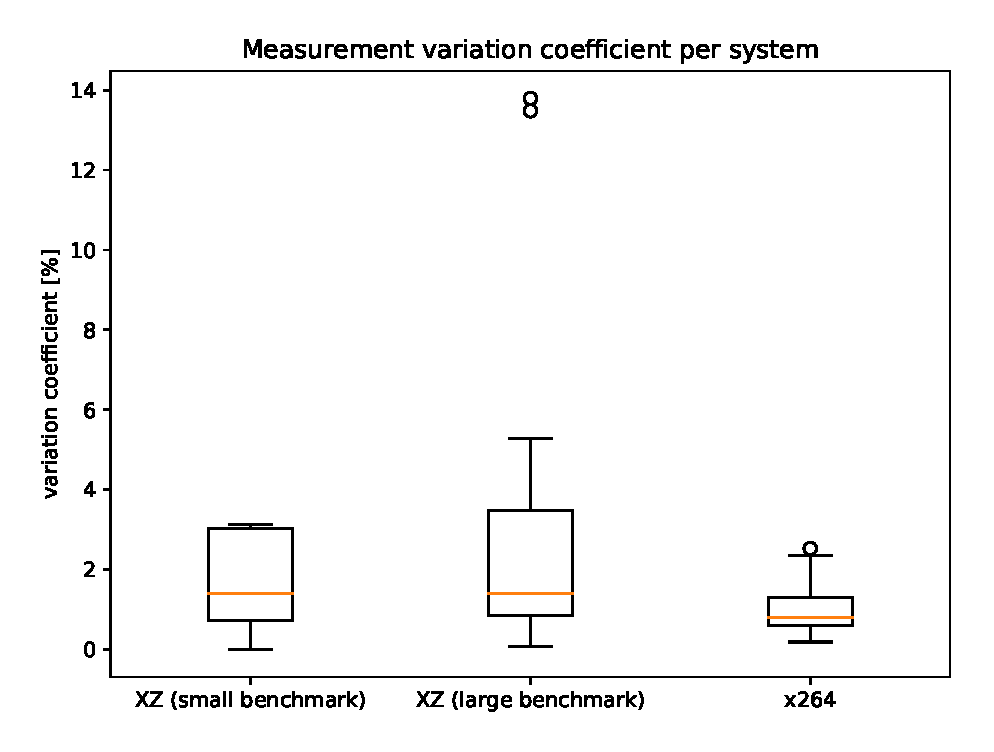
\includegraphics[width=0.48\textwidth]{images/reliability_1.eps}
 \end{center}
 \caption{Distributions of variation coefficients for
 GNU XZ (for two different benchmarks), and for x264.
 Measured median variation coefficients were
 1.408\,\% and 1.40\,\% for GNU XZ, and 0.794\,\% for
 x264.}\label{fig:reliability_1}
\end{wrapfigure}

For this experiment, of the two
sample system GNU XZ and x264, we selected three variants each. Each of the
three variants is derived from configuration presets with the incentive to
obtain a fast-,  medium-, and a slow-performing variant. The rationale behind this
approach is that conclusions about a configurable software system drawn from
multiple variants are more valid than simply measuring one arbitrary variant.
In addition, this choice allows us to investigate the influence of the
execution time on spread as we expect different levels of execution time
measurements. Each experiment was repeated three to 20 times. Finally, since
the execution time measurements for the Canterbury corpus for GNU XZ were
relatively small (around one second), we tested the same three variants with an
additional benchmark which is the Canterbury corpus tripled in size.

First, we investigated the influence of the configurable software system
studied. Therefore, in Figure\,\ref{fig:reliability_1}, we illustrate the
distribution of the variation coefficients for each experiment per system. The variation
coefficient is computed as the  standard deviation of the execution time divided
by (or normalized to) the arithmetic mean in order to compare the measures of
spread for arbitrary distributions. 
We see that for GNU XZ, regardless of the benchmark, the variation coefficient
is almost two times higher than for x264. This observation indicates, that for
GNU XZ, the execution time measurement variance is notably higher, suggesting
that the software system tested has an influence on how strongly measurements
can spread.

\begin{figure}
\centering
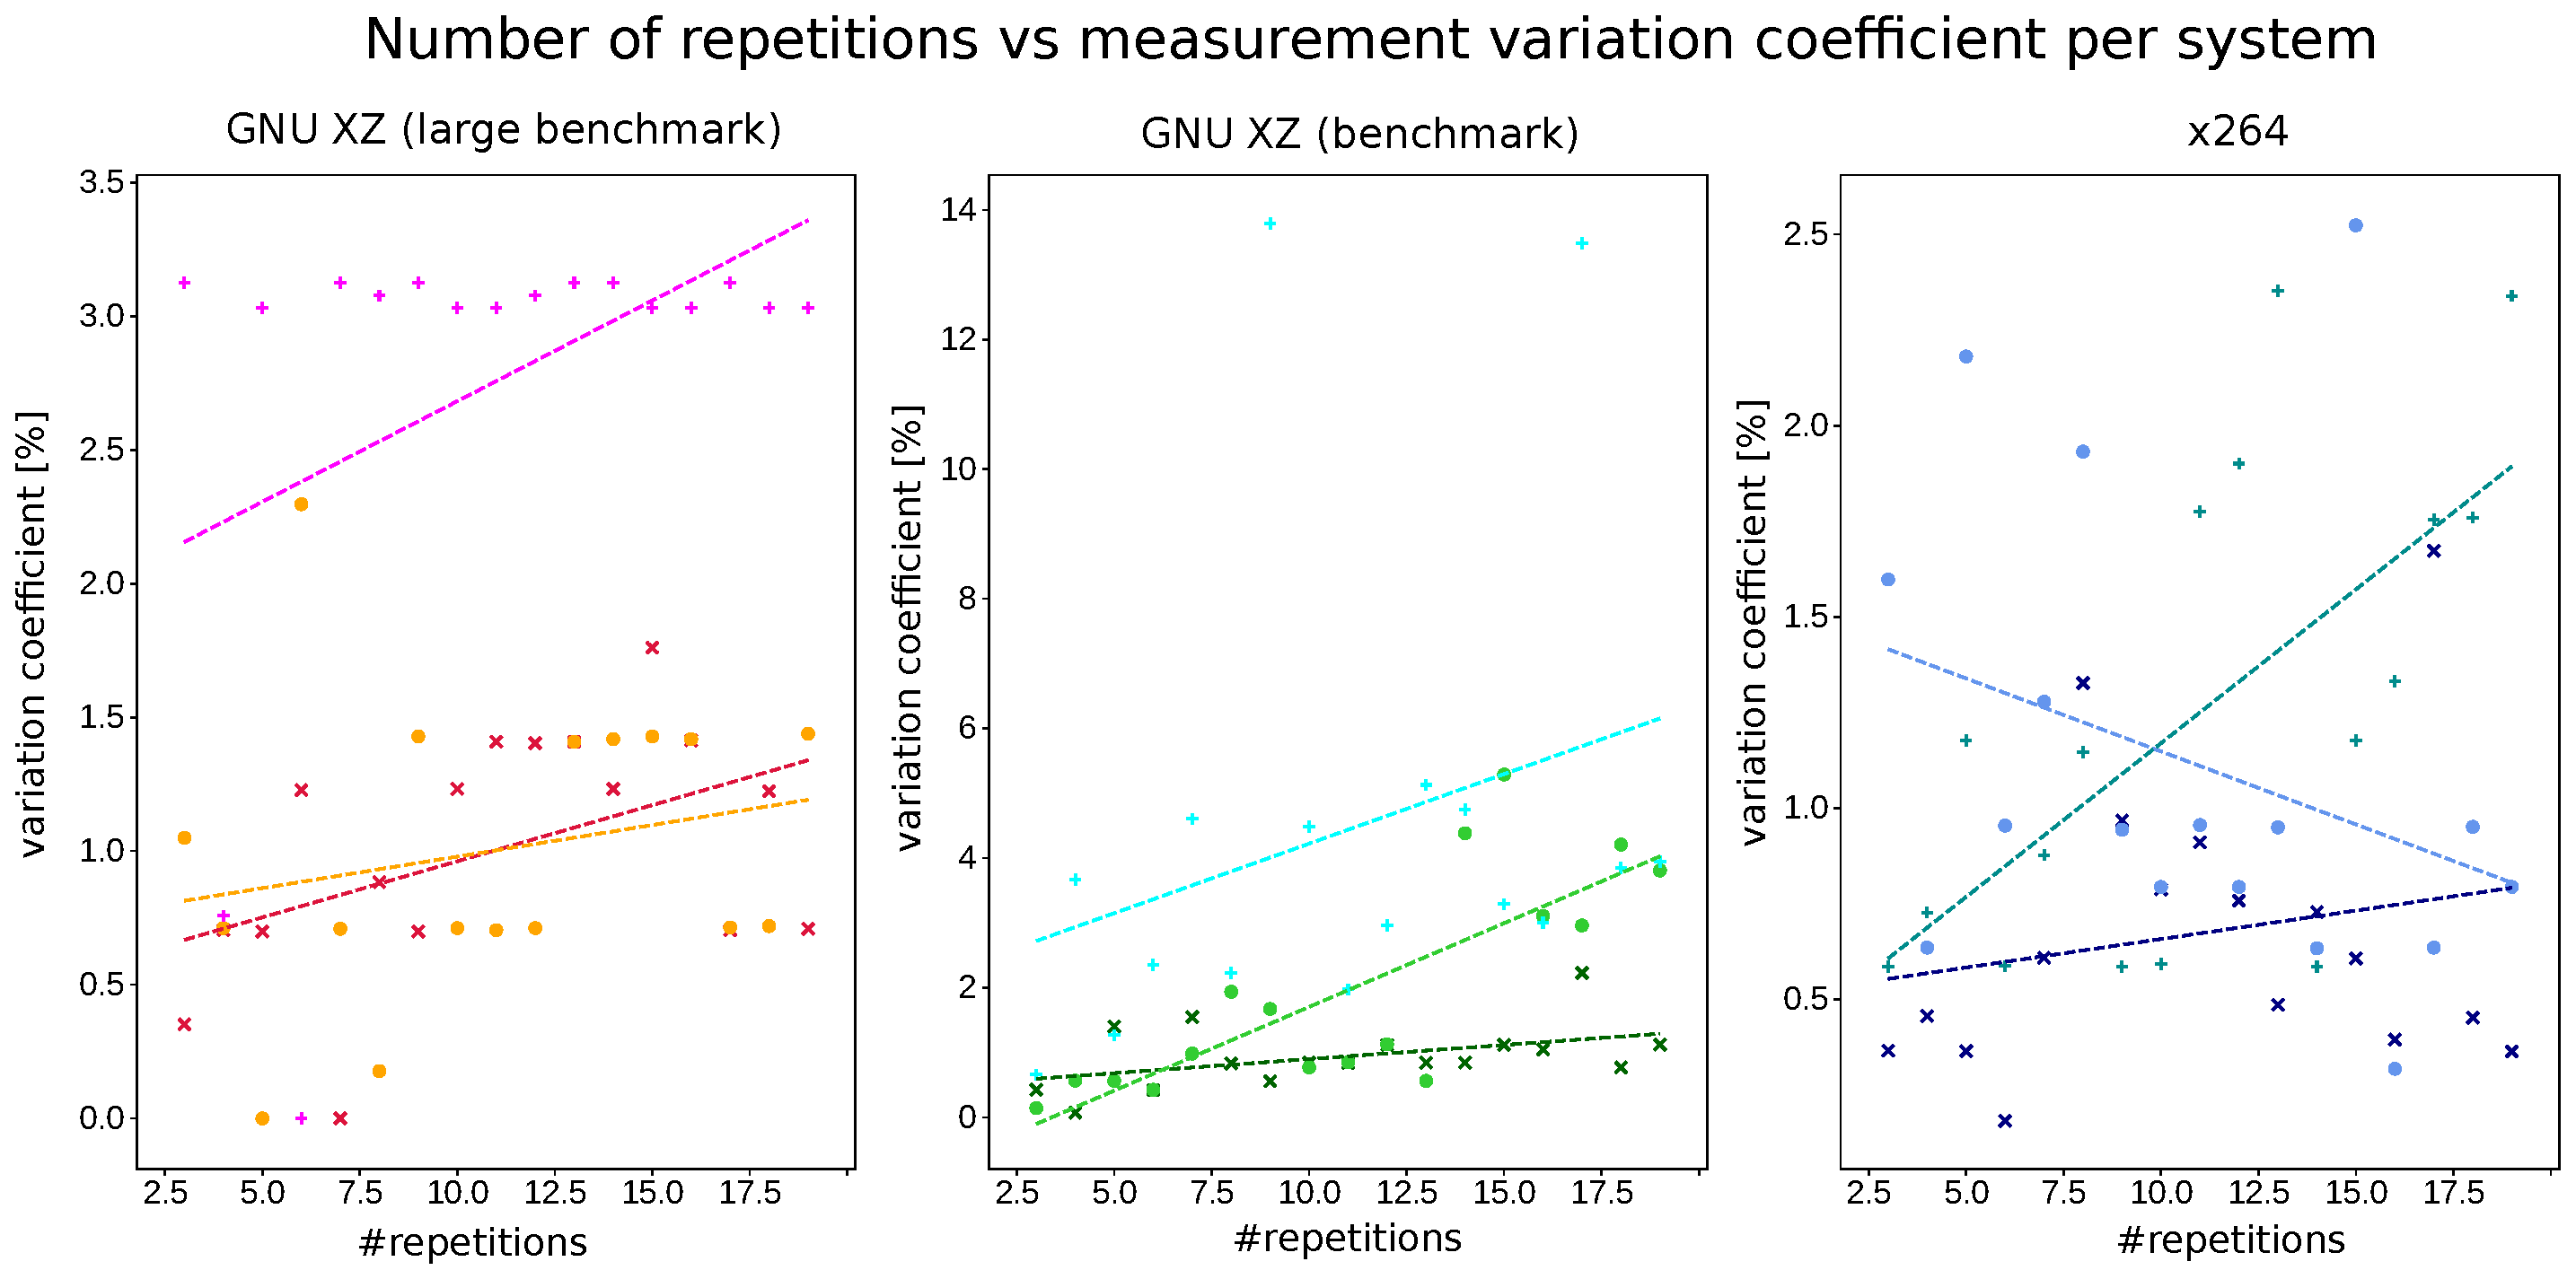
\includegraphics[width=0.99\textwidth]{images/reliability_3.eps}
\caption{Number of repetitions vs execution time measurement variation
coefficients for GNU XZ and x264. For GNU XZ, we tested two benchmarks
differing in size (the Canterbury corpus and a triple copy thereof). For each
subplot, we present three variants, one slow-, one medium-, and one
fast-performing one, each depicted by different colors and markers (\texttt{x}:
slow, \texttt{o}:medium, \texttt{+}: fast).}\label{fig:reliability_3}
\end{figure}

Second, we investigated the influence of the number of repetitions on the
variation coefficient of execution time measurements. In
Figure\,\ref{fig:reliability_3}, we illustrate the variation coefficients
plotted against the number of repetitions. We colorized each variant uniquely,
and assigned markers for each variant (\texttt{x} for the slow-,
{\texttt{o}} for the medium-, and \texttt{+} for the fast-performing variants).
In addition, we provided best linear fit curves of the same color to identify possible
trends. However, non of the presented fits suggests a significant relationship.

In conclusion, the only significant influence we could determine in our small
reliability assessment was the influence of the configurable software system
studied. The results suggest, that the software system studied influences the
reliability of execution time measurements. Further investigation, in particular
with regard to the question, what properties of a configurable software system
drive the impact on reliability, is required to determine the degree of
(non-)determinism of a configurable software system. However, this question
exceeds the scope of this thesis. All in all, we conclude that performance, or
execution time measurements using the unix \texttt{time} command are suffiently
reliable for the purpose of assessing the performance evolution of configurable
software systems.




%\chapter{Related Work}
%While to the best of our knowledge, there exists no previous work on
exhaustively presenting a methodology to understand and comprehend performance
evolution of configurable system, existing related work and ours have either
touched on similar topics, or pursue a similar methodology, yet with different
basic premises. In the following we present and summarize related work to
emphasize the limited scope of our work, and to give an outline of possible
future research directions.

\paragraph{Comprehending Software Evolution.} Throughout our methodology, we
have frequently referred to visualizations of data obtained from repository
mining, for instance, for commit activity, and as a basis for revision sampling
strategies. In addition, we have taken into account similar data in the
interpretation of our performance evolution history data in section. More
generally speaking, software as a product is the result of a complex
development process involving a repeatedly revised codebase, testing and
documentation activity as well as records of developer communication, and
organizational artifacts and speifications. As software evolves, hence, it is
inevitable to not consider those data to obtain more complete and integrated
insights. Aggregation and visualization of aforementioned data records can help
to sketch and understand possible coherences.

\cite{german_visualizing_2006} have presented a comprehensive tool,
\emph{softChange}, to visualize multiple aspects of a software system’s
evolution history, including commit and file activity graphs, authorship
overviews, and visualizations of file coupling. While their tool is not
designed with regard to a specific research direction, the authors stress the
importance of means to aggregate and analyze software trails in order to
explore and understand software evolution. Joint visualizations
of software trails as well as performance evolution history data is a promising
augmentation in the comprehension of multi-layered software evolution.

\cite{wu_exploring_2004} have presented presented an integrated approach to
visualize multiple different measurements over time. Their proposed
\emph{evolution spectrum graphs} are inspired by spectrum visualizations for
audio signals. A spectrum in their context can, for instance,  be a list of files, for which
different measurements are illustrated over time. While this approach allows a
global overview over an arbitrary timespan, it also can sketch fine-grained
changes and trends over time. Although, according to the authors, the
visualizations need to be tailored to the target system with respect to
coloring and spectrum selection, evolution spectrum graphs can be a useful
means to aggregate and visualize various single-valued measurements for a
spectrum of variants for configurable software systems.

To conclude with a broader overview on visualization tools for further reading,
\cite{storey_use_2005} have surveyed twelve tools (including the previously
mentioned two) that intend to visualize any kind of human activities in
software development with a string focus on software evolution. The authors
evaluate the different tools with respect to different aspects, including
intent of the tools, the information sources utilized by the tools, the form of
presentation offered by the tools, and the effectiveness in terms of
feasibility and validity.

\paragraph{Power Consumption as Performance Property.}
\begin{itemize}
  \item Awareness of power consumption as a quality property
  \citep{sahin_how_2014,li_empirical_2014}
  \item Methodology to power consumption assessment
  \citep{hindle_green_2015,hindle_greenminer:_2014}
\end{itemize}

\chapter{Conclusion}\label{chapter:7}
\clearpage

%\addcontentsline{toc}{chapter}{Bibliography} 
\bibliography{library}

\end{document}
